\documentclass[twoside]{book}

% Packages required by doxygen
\usepackage{fixltx2e}
\usepackage{calc}
\usepackage{doxygen}
\usepackage{graphicx}
\usepackage[utf8]{inputenc}
\usepackage{makeidx}
\usepackage{multicol}
\usepackage{multirow}
\PassOptionsToPackage{warn}{textcomp}
\usepackage{textcomp}
\usepackage[nointegrals]{wasysym}
\usepackage[table]{xcolor}

% Font selection
\usepackage[T1]{fontenc}
\usepackage{mathptmx}
\usepackage[scaled=.90]{helvet}
\usepackage{courier}
\usepackage{amssymb}
\usepackage{sectsty}
\renewcommand{\familydefault}{\sfdefault}
\allsectionsfont{%
  \fontseries{bc}\selectfont%
  \color{darkgray}%
}
\renewcommand{\DoxyLabelFont}{%
  \fontseries{bc}\selectfont%
  \color{darkgray}%
}
\newcommand{\+}{\discretionary{\mbox{\scriptsize$\hookleftarrow$}}{}{}}

% Page & text layout
\usepackage{geometry}
\geometry{%
  a4paper,%
  top=2.5cm,%
  bottom=2.5cm,%
  left=2.5cm,%
  right=2.5cm%
}
\tolerance=750
\hfuzz=15pt
\hbadness=750
\setlength{\emergencystretch}{15pt}
\setlength{\parindent}{0cm}
\setlength{\parskip}{0.2cm}
\makeatletter
\renewcommand{\paragraph}{%
  \@startsection{paragraph}{4}{0ex}{-1.0ex}{1.0ex}{%
    \normalfont\normalsize\bfseries\SS@parafont%
  }%
}
\renewcommand{\subparagraph}{%
  \@startsection{subparagraph}{5}{0ex}{-1.0ex}{1.0ex}{%
    \normalfont\normalsize\bfseries\SS@subparafont%
  }%
}
\makeatother

% Headers & footers
\usepackage{fancyhdr}
\pagestyle{fancyplain}
\fancyhead[LE]{\fancyplain{}{\bfseries\thepage}}
\fancyhead[CE]{\fancyplain{}{}}
\fancyhead[RE]{\fancyplain{}{\bfseries\leftmark}}
\fancyhead[LO]{\fancyplain{}{\bfseries\rightmark}}
\fancyhead[CO]{\fancyplain{}{}}
\fancyhead[RO]{\fancyplain{}{\bfseries\thepage}}
\fancyfoot[LE]{\fancyplain{}{}}
\fancyfoot[CE]{\fancyplain{}{}}
\fancyfoot[RE]{\fancyplain{}{\bfseries\scriptsize Generated on Thu Nov 27 2014 17\+:24\+:36 for S\+D\+L\+\_\+\+Assignment1 by Doxygen }}
\fancyfoot[LO]{\fancyplain{}{\bfseries\scriptsize Generated on Thu Nov 27 2014 17\+:24\+:36 for S\+D\+L\+\_\+\+Assignment1 by Doxygen }}
\fancyfoot[CO]{\fancyplain{}{}}
\fancyfoot[RO]{\fancyplain{}{}}
\renewcommand{\footrulewidth}{0.4pt}
\renewcommand{\chaptermark}[1]{%
  \markboth{#1}{}%
}
\renewcommand{\sectionmark}[1]{%
  \markright{\thesection\ #1}%
}

% Indices & bibliography
\usepackage{natbib}
\usepackage[titles]{tocloft}
\setcounter{tocdepth}{3}
\setcounter{secnumdepth}{5}
\makeindex

% Hyperlinks (required, but should be loaded last)
\usepackage{ifpdf}
\ifpdf
  \usepackage[pdftex,pagebackref=true]{hyperref}
\else
  \usepackage[ps2pdf,pagebackref=true]{hyperref}
\fi
\hypersetup{%
  colorlinks=true,%
  linkcolor=blue,%
  citecolor=blue,%
  unicode%
}

% Custom commands
\newcommand{\clearemptydoublepage}{%
  \newpage{\pagestyle{empty}\cleardoublepage}%
}


%===== C O N T E N T S =====

\begin{document}

% Titlepage & ToC
\hypersetup{pageanchor=false,
             bookmarks=true,
             bookmarksnumbered=true,
             pdfencoding=unicode
            }
\pagenumbering{roman}
\begin{titlepage}
\vspace*{7cm}
\begin{center}%
{\Large S\+D\+L\+\_\+\+Assignment1 }\\
\vspace*{1cm}
{\large Generated by Doxygen 1.8.8}\\
\vspace*{0.5cm}
{\small Thu Nov 27 2014 17:24:36}\\
\end{center}
\end{titlepage}
\clearemptydoublepage
\tableofcontents
\clearemptydoublepage
\pagenumbering{arabic}
\hypersetup{pageanchor=true}

%--- Begin generated contents ---
\chapter{Hierarchical Index}
\section{Class Hierarchy}
This inheritance list is sorted roughly, but not completely, alphabetically\+:\begin{DoxyCompactList}
\item \contentsline{section}{Animation}{\pageref{class_animation}}{}
\item \contentsline{section}{Application}{\pageref{class_application}}{}
\item \contentsline{section}{Background}{\pageref{class_background}}{}
\item \contentsline{section}{Entity}{\pageref{class_entity}}{}
\begin{DoxyCompactList}
\item \contentsline{section}{Moemon}{\pageref{class_moemon}}{}
\item \contentsline{section}{Player}{\pageref{class_player}}{}
\end{DoxyCompactList}
\item \contentsline{section}{Event\+Handler}{\pageref{class_event_handler}}{}
\item \contentsline{section}{File\+Loader}{\pageref{class_file_loader}}{}
\item \contentsline{section}{Load\+Texture}{\pageref{class_load_texture}}{}
\item \contentsline{section}{Rect}{\pageref{struct_rect}}{}
\item \contentsline{section}{Texture}{\pageref{class_texture}}{}
\item \contentsline{section}{Tile}{\pageref{class_tile}}{}
\item \contentsline{section}{Time}{\pageref{class_time}}{}
\item \contentsline{section}{Timer}{\pageref{class_timer}}{}
\item \contentsline{section}{Vec2}{\pageref{struct_vec2}}{}
\item \contentsline{section}{Vec4}{\pageref{struct_vec4}}{}
\end{DoxyCompactList}

\chapter{Class Index}
\section{Class List}
Here are the classes, structs, unions and interfaces with brief descriptions\+:\begin{DoxyCompactList}
\item\contentsline{section}{\hyperlink{class_animation}{Animation} }{\pageref{class_animation}}{}
\item\contentsline{section}{\hyperlink{class_application}{Application} \\*A class representing the \hyperlink{class_application}{Application} }{\pageref{class_application}}{}
\item\contentsline{section}{\hyperlink{class_background}{Background} \\*A class that represents a background }{\pageref{class_background}}{}
\item\contentsline{section}{\hyperlink{class_entity}{Entity} \\*A class that represents an \hyperlink{class_entity}{Entity} }{\pageref{class_entity}}{}
\item\contentsline{section}{\hyperlink{class_event_handler}{Event\+Handler} \\*A Class that represents the Event Handler }{\pageref{class_event_handler}}{}
\item\contentsline{section}{\hyperlink{class_file_loader}{File\+Loader} \\*A class that represents the \hyperlink{class_file_loader}{File\+Loader} }{\pageref{class_file_loader}}{}
\item\contentsline{section}{\hyperlink{class_load_texture}{Load\+Texture} \\*A class that represents a \hyperlink{class_texture}{Texture} Loader }{\pageref{class_load_texture}}{}
\item\contentsline{section}{\hyperlink{class_moemon}{Moemon} \\*Class that represents an Moe\+Mon }{\pageref{class_moemon}}{}
\item\contentsline{section}{\hyperlink{class_player}{Player} \\*A class that represents a \hyperlink{class_player}{Player} }{\pageref{class_player}}{}
\item\contentsline{section}{\hyperlink{struct_rect}{Rect} \\*A structure containing four floats }{\pageref{struct_rect}}{}
\item\contentsline{section}{\hyperlink{class_texture}{Texture} }{\pageref{class_texture}}{}
\item\contentsline{section}{\hyperlink{class_tile}{Tile} \\*A class that represents a \hyperlink{class_tile}{Tile} }{\pageref{class_tile}}{}
\item\contentsline{section}{\hyperlink{class_time}{Time} \\*A class that represents time }{\pageref{class_time}}{}
\item\contentsline{section}{\hyperlink{class_timer}{Timer} \\*A class that represents a timer }{\pageref{class_timer}}{}
\item\contentsline{section}{\hyperlink{struct_vec2}{Vec2} \\*A structure that represents a Vector of 2 dimensions }{\pageref{struct_vec2}}{}
\item\contentsline{section}{\hyperlink{struct_vec4}{Vec4} }{\pageref{struct_vec4}}{}
\end{DoxyCompactList}

\chapter{Class Documentation}
\hypertarget{class_animation}{\section{Animation Class Reference}
\label{class_animation}\index{Animation@{Animation}}
}
\subsection*{Public Member Functions}
\begin{DoxyCompactItemize}
\item 
\hypertarget{class_animation_a925d01846cf36477cdf1396fc8491c2a}{void {\bfseries on\+Animation} ()}\label{class_animation_a925d01846cf36477cdf1396fc8491c2a}

\item 
\hypertarget{class_animation_a766f27c5185d8a40ac8212fff70483ce}{void {\bfseries set\+Frame\+Rate} (int i\+Rate)}\label{class_animation_a766f27c5185d8a40ac8212fff70483ce}

\item 
\hypertarget{class_animation_a6d5cb157fa9676c6d46325714ab67d1d}{void {\bfseries set\+Current\+Frame} (int i\+Frame)}\label{class_animation_a6d5cb157fa9676c6d46325714ab67d1d}

\item 
\hypertarget{class_animation_af83ac9868e12f12ec252e63bb20fec70}{int {\bfseries Get\+Current\+Frame} ()}\label{class_animation_af83ac9868e12f12ec252e63bb20fec70}

\end{DoxyCompactItemize}
\subsection*{Public Attributes}
\begin{DoxyCompactItemize}
\item 
\hypertarget{class_animation_aa28d390bb19cb71a6390e117d921568a}{int {\bfseries i\+Max\+Frames}}\label{class_animation_aa28d390bb19cb71a6390e117d921568a}

\item 
\hypertarget{class_animation_a65426691a609d287408f32f27305a5c1}{bool {\bfseries bfluctuate}}\label{class_animation_a65426691a609d287408f32f27305a5c1}

\end{DoxyCompactItemize}
\subsection*{Protected Attributes}
\begin{DoxyCompactItemize}
\item 
\hypertarget{class_animation_aa08785d681ca1561a8993a4e2b6836dd}{int {\bfseries i\+Current\+Frame}}\label{class_animation_aa08785d681ca1561a8993a4e2b6836dd}

\item 
\hypertarget{class_animation_a37a404d5332f5a1cfdcbbf4b2266f6df}{int {\bfseries i\+Frame\+Increment}}\label{class_animation_a37a404d5332f5a1cfdcbbf4b2266f6df}

\item 
\hypertarget{class_animation_a13a8758598d83105912bf2dc28fb6e74}{int {\bfseries i\+Frame\+Rate}}\label{class_animation_a13a8758598d83105912bf2dc28fb6e74}

\item 
\hypertarget{class_animation_a97892a7f4ed270540edc4ad298370d8a}{long {\bfseries l\+Past\+Time}}\label{class_animation_a97892a7f4ed270540edc4ad298370d8a}

\end{DoxyCompactItemize}


The documentation for this class was generated from the following files\+:\begin{DoxyCompactItemize}
\item 
S\+D\+L/Animation.\+h\item 
S\+D\+L/Animation.\+cpp\end{DoxyCompactItemize}

\hypertarget{class_application}{\section{Application Class Reference}
\label{class_application}\index{Application@{Application}}
}


A class representing the \hyperlink{class_application}{Application}.  




{\ttfamily \#include $<$Application.\+h$>$}

\subsection*{Public Member Functions}
\begin{DoxyCompactItemize}
\item 
\hypertarget{class_application_afa8cc05ce6b6092be5ecdfdae44e05f8}{\hyperlink{class_application_afa8cc05ce6b6092be5ecdfdae44e05f8}{Application} ()}\label{class_application_afa8cc05ce6b6092be5ecdfdae44e05f8}

\begin{DoxyCompactList}\small\item\em The default constructor. \end{DoxyCompactList}\item 
\hypertarget{class_application_a748bca84fefb9c12661cfaa2f623748d}{\hyperlink{class_application_a748bca84fefb9c12661cfaa2f623748d}{$\sim$\+Application} ()}\label{class_application_a748bca84fefb9c12661cfaa2f623748d}

\begin{DoxyCompactList}\small\item\em The default deconstructor. \end{DoxyCompactList}\item 
bool \hyperlink{class_application_afabe70d81db4451db19d267b3e47953c}{call\+Init} ()
\begin{DoxyCompactList}\small\item\em A method to call Initialisation. \end{DoxyCompactList}\item 
int \hyperlink{class_application_aae6cea757aa072af2b04f80f0dc43035}{call\+Execution} ()
\begin{DoxyCompactList}\small\item\em A method to call execution. \end{DoxyCompactList}\item 
void \hyperlink{class_application_a120691d97bf8c56542863cfb629c5334}{call\+Event} (S\+D\+L\+\_\+\+Event $\ast$sdl\+Event)
\begin{DoxyCompactList}\small\item\em A method that is called as part of the game loop. \end{DoxyCompactList}\item 
void \hyperlink{class_application_ac45e87c4784cb82521166105137147ee}{call\+Loop} ()
\begin{DoxyCompactList}\small\item\em A method that is called as part of the game loop. \end{DoxyCompactList}\item 
void \hyperlink{class_application_a8164c003d80f4ac88300a3b972abf259}{call\+Renderer} ()
\begin{DoxyCompactList}\small\item\em A method to call the rendering function. \end{DoxyCompactList}\item 
void \hyperlink{class_application_aa85cb7c4c0ba25070aa3320618b04821}{call\+Cleanup} ()
\begin{DoxyCompactList}\small\item\em This method is called when the program exits. \end{DoxyCompactList}\item 
void \hyperlink{class_application_a2d00469b8187f560ba9ff8574a1e2477}{call\+Surface} ()
\begin{DoxyCompactList}\small\item\em A method to set the surface of all visual objects. \end{DoxyCompactList}\item 
void \hyperlink{class_application_a185d7edc1ca8c5f9ca86fd927a486848}{call\+Texture} ()
\begin{DoxyCompactList}\small\item\em A method to set the texture of all visual objects. \end{DoxyCompactList}\end{DoxyCompactItemize}
\subsection*{Protected Attributes}
\begin{DoxyCompactItemize}
\item 
\hypertarget{class_application_ac6112748a352677fa369ead5e3fd7b53}{bool \hyperlink{class_application_ac6112748a352677fa369ead5e3fd7b53}{Game\+Loop}}\label{class_application_ac6112748a352677fa369ead5e3fd7b53}

\begin{DoxyCompactList}\small\item\em A bool to start or end the game loop. \end{DoxyCompactList}\item 
\hypertarget{class_application_a9216c8c03870932d081b5e6fe33e21a8}{S\+D\+L\+\_\+\+Window $\ast$ \hyperlink{class_application_a9216c8c03870932d081b5e6fe33e21a8}{Display}}\label{class_application_a9216c8c03870932d081b5e6fe33e21a8}

\begin{DoxyCompactList}\small\item\em A S\+D\+L\+\_\+\+Window$\ast$ for creating the screen. \end{DoxyCompactList}\item 
\hypertarget{class_application_a6ebb16ce7358f874306c3593fd3abd39}{\hyperlink{class_file_loader}{File\+Loader} $\ast$ \hyperlink{class_application_a6ebb16ce7358f874306c3593fd3abd39}{f\+Loader}}\label{class_application_a6ebb16ce7358f874306c3593fd3abd39}

\begin{DoxyCompactList}\small\item\em A \hyperlink{class_file_loader}{File\+Loader} object for loading in the different files required. \end{DoxyCompactList}\item 
\hypertarget{class_application_aa164b18de54da4097c294b96f65e5dd1}{std\+::vector$<$ \hyperlink{class_moemon}{Moemon} $>$ \hyperlink{class_application_aa164b18de54da4097c294b96f65e5dd1}{Moe\+Mon\+List}}\label{class_application_aa164b18de54da4097c294b96f65e5dd1}

\begin{DoxyCompactList}\small\item\em A vector of \hyperlink{class_moemon}{Moemon} that stores all the \hyperlink{class_moemon}{Moemon} the application will use. \end{DoxyCompactList}\item 
\hypertarget{class_application_a5066daff6377e8577b11ff6706fef9bb}{\hyperlink{class_player}{Player} $\ast$ \hyperlink{class_application_a5066daff6377e8577b11ff6706fef9bb}{Player\+Entity}}\label{class_application_a5066daff6377e8577b11ff6706fef9bb}

\begin{DoxyCompactList}\small\item\em A \hyperlink{class_player}{Player} object. \end{DoxyCompactList}\item 
\hypertarget{class_application_a4678ca860a3791b2d09ef777fbdb3167}{\hyperlink{class_background}{Background} $\ast$ \hyperlink{class_application_a4678ca860a3791b2d09ef777fbdb3167}{Backgrounds}}\label{class_application_a4678ca860a3791b2d09ef777fbdb3167}

\begin{DoxyCompactList}\small\item\em A background object (subject to change) \end{DoxyCompactList}\item 
\hypertarget{class_application_af90aee2b6a03b1b1b1d7b9f06b622585}{S\+D\+L\+\_\+\+Renderer $\ast$ \hyperlink{class_application_af90aee2b6a03b1b1b1d7b9f06b622585}{Renderer}}\label{class_application_af90aee2b6a03b1b1b1d7b9f06b622585}

\begin{DoxyCompactList}\small\item\em The S\+D\+L\+\_\+\+Renderer used to render textures to the screen. \end{DoxyCompactList}\item 
\hypertarget{class_application_a9a357975280488b775fda3f363ec556d}{\hyperlink{class_load_texture}{Load\+Texture} $\ast$ \hyperlink{class_application_a9a357975280488b775fda3f363ec556d}{Texture\+Loader}}\label{class_application_a9a357975280488b775fda3f363ec556d}

\begin{DoxyCompactList}\small\item\em A \hyperlink{class_load_texture}{Load\+Texture} object for loading in the surface/textures. \end{DoxyCompactList}\item 
\hypertarget{class_application_a5b3b987a58f1ff2cd672c52f05a46b2f}{\hyperlink{class_time}{Time} \hyperlink{class_application_a5b3b987a58f1ff2cd672c52f05a46b2f}{time}}\label{class_application_a5b3b987a58f1ff2cd672c52f05a46b2f}

\begin{DoxyCompactList}\small\item\em A time object for managing delta time. \end{DoxyCompactList}\item 
\hypertarget{class_application_a31d4246ee49a814ca3110f3e51ccd03f}{\hyperlink{class_event_handler}{Event\+Handler} $\ast$ \hyperlink{class_application_a31d4246ee49a814ca3110f3e51ccd03f}{Event}}\label{class_application_a31d4246ee49a814ca3110f3e51ccd03f}

\begin{DoxyCompactList}\small\item\em A \hyperlink{class_event_handler}{Event\+Handler} object. \end{DoxyCompactList}\item 
\hypertarget{class_application_aad86b8086daa8c8d85e803aa7f3b70da}{const int \hyperlink{class_application_aad86b8086daa8c8d85e803aa7f3b70da}{W\+I\+N\+D\+O\+W\+\_\+\+X} = 100}\label{class_application_aad86b8086daa8c8d85e803aa7f3b70da}

\begin{DoxyCompactList}\small\item\em A constant int for the window's x axises. \end{DoxyCompactList}\item 
\hypertarget{class_application_a44acc475d3da03e92d09629cc88bfffb}{const int \hyperlink{class_application_a44acc475d3da03e92d09629cc88bfffb}{W\+I\+N\+D\+O\+W\+\_\+\+Y} = 100}\label{class_application_a44acc475d3da03e92d09629cc88bfffb}

\begin{DoxyCompactList}\small\item\em A constant int for the window's y axises. \end{DoxyCompactList}\item 
\hypertarget{class_application_a58027269bdd05739a498f4e35d36380c}{const int \hyperlink{class_application_a58027269bdd05739a498f4e35d36380c}{W\+I\+N\+D\+O\+W\+\_\+\+W\+I\+D\+T\+H} = 640}\label{class_application_a58027269bdd05739a498f4e35d36380c}

\begin{DoxyCompactList}\small\item\em A constant int for the window's Width. \end{DoxyCompactList}\item 
\hypertarget{class_application_a0bfec21f44d9cd3972fadf5ab5485e3b}{const int \hyperlink{class_application_a0bfec21f44d9cd3972fadf5ab5485e3b}{W\+I\+N\+D\+O\+W\+\_\+\+H\+E\+I\+G\+H\+T} = 480}\label{class_application_a0bfec21f44d9cd3972fadf5ab5485e3b}

\begin{DoxyCompactList}\small\item\em A constant int for the window's Height. \end{DoxyCompactList}\end{DoxyCompactItemize}


\subsection{Detailed Description}
A class representing the \hyperlink{class_application}{Application}. 

Contains the methods, and parameters that build up the application. Contains the application and use of all class objects. 

\subsection{Member Function Documentation}
\hypertarget{class_application_aa85cb7c4c0ba25070aa3320618b04821}{\index{Application@{Application}!call\+Cleanup@{call\+Cleanup}}
\index{call\+Cleanup@{call\+Cleanup}!Application@{Application}}
\subsubsection[{call\+Cleanup}]{\setlength{\rightskip}{0pt plus 5cm}void Application\+::call\+Cleanup (
\begin{DoxyParamCaption}
{}
\end{DoxyParamCaption}
)}}\label{class_application_aa85cb7c4c0ba25070aa3320618b04821}


This method is called when the program exits. 

This method cleans up all the vectors, objects, and any other parts of the application before exiting. \hypertarget{class_application_a120691d97bf8c56542863cfb629c5334}{\index{Application@{Application}!call\+Event@{call\+Event}}
\index{call\+Event@{call\+Event}!Application@{Application}}
\subsubsection[{call\+Event}]{\setlength{\rightskip}{0pt plus 5cm}void Application\+::call\+Event (
\begin{DoxyParamCaption}
\item[{S\+D\+L\+\_\+\+Event $\ast$}]{sdl\+Event}
\end{DoxyParamCaption}
)}}\label{class_application_a120691d97bf8c56542863cfb629c5334}


A method that is called as part of the game loop. 

This method takes in the event parameter, and manages the \hyperlink{class_event_handler}{Event\+Handler} object.


\begin{DoxyParams}{Parameters}
{\em S\+D\+L\+\_\+\+Event$\ast$} & -\/ A S\+D\+L\+\_\+\+Event$\ast$ that contains all the events that S\+D\+L catches \\
\hline
\end{DoxyParams}
\begin{DoxyReturn}{Returns}
0 
\end{DoxyReturn}
\hypertarget{class_application_aae6cea757aa072af2b04f80f0dc43035}{\index{Application@{Application}!call\+Execution@{call\+Execution}}
\index{call\+Execution@{call\+Execution}!Application@{Application}}
\subsubsection[{call\+Execution}]{\setlength{\rightskip}{0pt plus 5cm}int Application\+::call\+Execution (
\begin{DoxyParamCaption}
{}
\end{DoxyParamCaption}
)}}\label{class_application_aae6cea757aa072af2b04f80f0dc43035}


A method to call execution. 

This method executes the main game loop, and the event handler. \begin{DoxyReturn}{Returns}
bool -\/ If the application has successfully initialised 
\end{DoxyReturn}
\hypertarget{class_application_afabe70d81db4451db19d267b3e47953c}{\index{Application@{Application}!call\+Init@{call\+Init}}
\index{call\+Init@{call\+Init}!Application@{Application}}
\subsubsection[{call\+Init}]{\setlength{\rightskip}{0pt plus 5cm}bool Application\+::call\+Init (
\begin{DoxyParamCaption}
{}
\end{DoxyParamCaption}
)}}\label{class_application_afabe70d81db4451db19d267b3e47953c}


A method to call Initialisation. 

This method initialises all the classes, and objects that are needed before the application loop begins. This is the very first method called on the application starting. \hypertarget{class_application_ac45e87c4784cb82521166105137147ee}{\index{Application@{Application}!call\+Loop@{call\+Loop}}
\index{call\+Loop@{call\+Loop}!Application@{Application}}
\subsubsection[{call\+Loop}]{\setlength{\rightskip}{0pt plus 5cm}void Application\+::call\+Loop (
\begin{DoxyParamCaption}
{}
\end{DoxyParamCaption}
)}}\label{class_application_ac45e87c4784cb82521166105137147ee}


A method that is called as part of the game loop. 

This method is where the methods of other objects are called to update them. \hyperlink{class_time}{Time} is updated here. \hypertarget{class_application_a8164c003d80f4ac88300a3b972abf259}{\index{Application@{Application}!call\+Renderer@{call\+Renderer}}
\index{call\+Renderer@{call\+Renderer}!Application@{Application}}
\subsubsection[{call\+Renderer}]{\setlength{\rightskip}{0pt plus 5cm}void Application\+::call\+Renderer (
\begin{DoxyParamCaption}
{}
\end{DoxyParamCaption}
)}}\label{class_application_a8164c003d80f4ac88300a3b972abf259}


A method to call the rendering function. 

This method is where the texture of objects are sent to the renderer. \hypertarget{class_application_a2d00469b8187f560ba9ff8574a1e2477}{\index{Application@{Application}!call\+Surface@{call\+Surface}}
\index{call\+Surface@{call\+Surface}!Application@{Application}}
\subsubsection[{call\+Surface}]{\setlength{\rightskip}{0pt plus 5cm}void Application\+::call\+Surface (
\begin{DoxyParamCaption}
{}
\end{DoxyParamCaption}
)}}\label{class_application_a2d00469b8187f560ba9ff8574a1e2477}


A method to set the surface of all visual objects. 

This method is where all the different objects that need surfaces are processed. This is called in the call\+Init method. \hypertarget{class_application_a185d7edc1ca8c5f9ca86fd927a486848}{\index{Application@{Application}!call\+Texture@{call\+Texture}}
\index{call\+Texture@{call\+Texture}!Application@{Application}}
\subsubsection[{call\+Texture}]{\setlength{\rightskip}{0pt plus 5cm}void Application\+::call\+Texture (
\begin{DoxyParamCaption}
{}
\end{DoxyParamCaption}
)}}\label{class_application_a185d7edc1ca8c5f9ca86fd927a486848}


A method to set the texture of all visual objects. 

This method is where all the different objects that need textures are processed. This is called in the call\+Init method. 

The documentation for this class was generated from the following files\+:\begin{DoxyCompactItemize}
\item 
S\+D\+L/Application.\+h\item 
S\+D\+L/Application.\+cpp\end{DoxyCompactItemize}

\hypertarget{class_background}{\section{Background Class Reference}
\label{class_background}\index{Background@{Background}}
}


A class that represents a background.  




{\ttfamily \#include $<$Background.\+h$>$}

\subsection*{Public Member Functions}
\begin{DoxyCompactItemize}
\item 
S\+D\+L\+\_\+\+Surface $\ast$ \hyperlink{class_background_ab0b25086c8d80f30ba80949ae9b81af6}{get\+Surface} ()
\begin{DoxyCompactList}\small\item\em A method to get the background surface. \end{DoxyCompactList}\item 
void \hyperlink{class_background_a0ba0f788a998021c2e93ceca3fe427e7}{set\+Surface} (S\+D\+L\+\_\+\+Surface $\ast$s\+Surface)
\begin{DoxyCompactList}\small\item\em A method to set the background surface. \end{DoxyCompactList}\item 
S\+D\+L\+\_\+\+Texture $\ast$ \hyperlink{class_background_ae335b7a3476558ac7231963e9a71c6f0}{get\+Texture} ()
\begin{DoxyCompactList}\small\item\em A method to get the background texture. \end{DoxyCompactList}\item 
void \hyperlink{class_background_a02480d048c8a5e7a915063ade9de9e8b}{set\+Texture} (S\+D\+L\+\_\+\+Texture $\ast$s\+Texture)
\begin{DoxyCompactList}\small\item\em A method to set the background texture. \end{DoxyCompactList}\item 
S\+D\+L\+\_\+\+Rect \hyperlink{class_background_a3005aceaae7861318581994a4961c99d}{get\+Rect} ()
\begin{DoxyCompactList}\small\item\em A method to get the background \hyperlink{struct_rect}{Rect}. \end{DoxyCompactList}\end{DoxyCompactItemize}


\subsection{Detailed Description}
A class that represents a background. 

This class is used to create a background object 

\subsection{Member Function Documentation}
\hypertarget{class_background_a3005aceaae7861318581994a4961c99d}{\index{Background@{Background}!get\+Rect@{get\+Rect}}
\index{get\+Rect@{get\+Rect}!Background@{Background}}
\subsubsection[{get\+Rect}]{\setlength{\rightskip}{0pt plus 5cm}S\+D\+L\+\_\+\+Rect Background\+::get\+Rect (
\begin{DoxyParamCaption}
{}
\end{DoxyParamCaption}
)}}\label{class_background_a3005aceaae7861318581994a4961c99d}


A method to get the background \hyperlink{struct_rect}{Rect}. 

Returns a S\+D\+L\+\_\+\+Rect when called. \hypertarget{class_background_ab0b25086c8d80f30ba80949ae9b81af6}{\index{Background@{Background}!get\+Surface@{get\+Surface}}
\index{get\+Surface@{get\+Surface}!Background@{Background}}
\subsubsection[{get\+Surface}]{\setlength{\rightskip}{0pt plus 5cm}S\+D\+L\+\_\+\+Surface $\ast$ Background\+::get\+Surface (
\begin{DoxyParamCaption}
{}
\end{DoxyParamCaption}
)}}\label{class_background_ab0b25086c8d80f30ba80949ae9b81af6}


A method to get the background surface. 

Returns a S\+D\+L\+\_\+\+Surface$\ast$ when called. \hypertarget{class_background_ae335b7a3476558ac7231963e9a71c6f0}{\index{Background@{Background}!get\+Texture@{get\+Texture}}
\index{get\+Texture@{get\+Texture}!Background@{Background}}
\subsubsection[{get\+Texture}]{\setlength{\rightskip}{0pt plus 5cm}S\+D\+L\+\_\+\+Texture $\ast$ Background\+::get\+Texture (
\begin{DoxyParamCaption}
{}
\end{DoxyParamCaption}
)}}\label{class_background_ae335b7a3476558ac7231963e9a71c6f0}


A method to get the background texture. 

Returns a S\+D\+L\+\_\+\+Texture$\ast$ when called. \hypertarget{class_background_a0ba0f788a998021c2e93ceca3fe427e7}{\index{Background@{Background}!set\+Surface@{set\+Surface}}
\index{set\+Surface@{set\+Surface}!Background@{Background}}
\subsubsection[{set\+Surface}]{\setlength{\rightskip}{0pt plus 5cm}void Background\+::set\+Surface (
\begin{DoxyParamCaption}
\item[{S\+D\+L\+\_\+\+Surface $\ast$}]{s\+Surface}
\end{DoxyParamCaption}
)}}\label{class_background_a0ba0f788a998021c2e93ceca3fe427e7}


A method to set the background surface. 

Takes a S\+D\+L\+\_\+\+Surface$\ast$ parameter, and sets the background Surface to it.


\begin{DoxyParams}{Parameters}
{\em S\+D\+L\+\_\+\+Surface$\ast$} & -\/ A S\+D\+L\+\_\+\+Surface$\ast$ that contains the background image. \\
\hline
\end{DoxyParams}
\begin{DoxyReturn}{Returns}
S\+D\+L\+\_\+\+Surface$\ast$ 
\end{DoxyReturn}
\hypertarget{class_background_a02480d048c8a5e7a915063ade9de9e8b}{\index{Background@{Background}!set\+Texture@{set\+Texture}}
\index{set\+Texture@{set\+Texture}!Background@{Background}}
\subsubsection[{set\+Texture}]{\setlength{\rightskip}{0pt plus 5cm}void Background\+::set\+Texture (
\begin{DoxyParamCaption}
\item[{S\+D\+L\+\_\+\+Texture $\ast$}]{s\+Texture}
\end{DoxyParamCaption}
)}}\label{class_background_a02480d048c8a5e7a915063ade9de9e8b}


A method to set the background texture. 

Takes a S\+D\+L\+\_\+\+Texture$\ast$ parameter, and sets the background texture to it.


\begin{DoxyParams}{Parameters}
{\em S\+D\+L\+\_\+\+Texture$\ast$} & -\/ A S\+D\+L\+\_\+\+Texture$\ast$ that contains a texture created from the surface \\
\hline
\end{DoxyParams}
\begin{DoxyReturn}{Returns}
S\+D\+L\+\_\+\+Texture$\ast$ 
\end{DoxyReturn}


The documentation for this class was generated from the following files\+:\begin{DoxyCompactItemize}
\item 
S\+D\+L/Background.\+h\item 
S\+D\+L/Background.\+cpp\end{DoxyCompactItemize}

\hypertarget{class_entity}{\section{Entity Class Reference}
\label{class_entity}\index{Entity@{Entity}}
}


A class that represents an \hyperlink{class_entity}{Entity}.  




{\ttfamily \#include $<$Entity.\+h$>$}

Inheritance diagram for Entity\+:\begin{figure}[H]
\begin{center}
\leavevmode
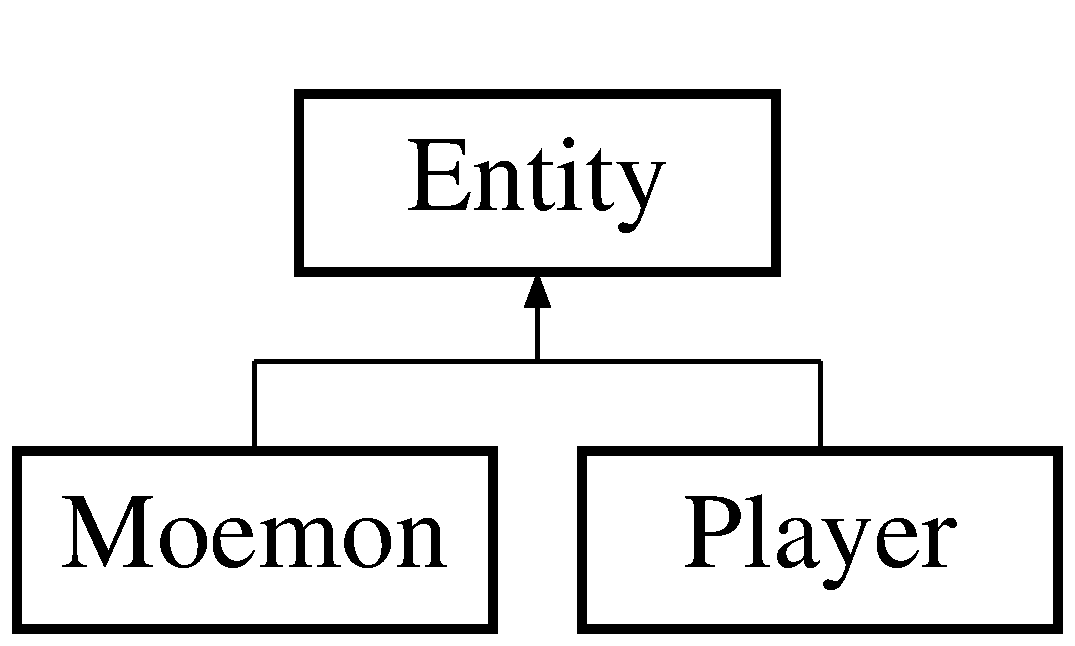
\includegraphics[height=2.000000cm]{class_entity}
\end{center}
\end{figure}
\subsection*{Public Member Functions}
\begin{DoxyCompactItemize}
\item 
\hyperlink{class_entity_a980f368aa07ce358583982821533a54a}{Entity} ()
\begin{DoxyCompactList}\small\item\em Constructs an \hyperlink{class_entity}{Entity} object. \end{DoxyCompactList}\item 
\hyperlink{class_entity_adf6d3f7cb1b2ba029b6b048a395cc8ae}{$\sim$\+Entity} ()
\begin{DoxyCompactList}\small\item\em Deconstructs an \hyperlink{class_entity}{Entity} object. \end{DoxyCompactList}\item 
void \hyperlink{class_entity_a67a6fb32075b44c055f20b9332068cf8}{set\+Surface} (S\+D\+L\+\_\+\+Surface $\ast$)
\begin{DoxyCompactList}\small\item\em A method to set the surface of the object. \end{DoxyCompactList}\item 
void \hyperlink{class_entity_aaae0b0b28be4497af93cf2277662770b}{set\+Texture} (S\+D\+L\+\_\+\+Texture $\ast$)
\begin{DoxyCompactList}\small\item\em A method to set the texture of the object. \end{DoxyCompactList}\item 
S\+D\+L\+\_\+\+Surface $\ast$ \hyperlink{class_entity_a3544323cdb2083bedbfa7f04e5cdaecf}{get\+Surface} ()
\begin{DoxyCompactList}\small\item\em A method to get the surface from the object. \end{DoxyCompactList}\item 
S\+D\+L\+\_\+\+Texture $\ast$ \hyperlink{class_entity_a25b50625a770e24dcafc25aa505fc54d}{get\+Texture} ()
\begin{DoxyCompactList}\small\item\em A method to get the texture from the object. \end{DoxyCompactList}\item 
S\+D\+L\+\_\+\+Rect \hyperlink{class_entity_ae113498b7c37c80a814f0d92444ebf50}{get\+Desc\+Rect} ()
\begin{DoxyCompactList}\small\item\em A method to get the Destination \hyperlink{struct_rect}{Rect}. \end{DoxyCompactList}\item 
S\+D\+L\+\_\+\+Rect \hyperlink{class_entity_a85faf9891defd68e4404178cc79a6419}{get\+Src\+Rect} ()
\begin{DoxyCompactList}\small\item\em A method to get the Source \hyperlink{struct_rect}{Rect}. \end{DoxyCompactList}\end{DoxyCompactItemize}
\subsection*{Protected Attributes}
\begin{DoxyCompactItemize}
\item 
\hypertarget{class_entity_a195e44184fd33d919f727ae93c18b9de}{S\+D\+L\+\_\+\+Surface $\ast$ \hyperlink{class_entity_a195e44184fd33d919f727ae93c18b9de}{Entity\+Surface}}\label{class_entity_a195e44184fd33d919f727ae93c18b9de}

\begin{DoxyCompactList}\small\item\em The objects Surface used to create a texture. \end{DoxyCompactList}\item 
\hypertarget{class_entity_a2dc0bd74bf1e764381adf09f4e0ac7a2}{S\+D\+L\+\_\+\+Texture $\ast$ \hyperlink{class_entity_a2dc0bd74bf1e764381adf09f4e0ac7a2}{Entity\+Texture}}\label{class_entity_a2dc0bd74bf1e764381adf09f4e0ac7a2}

\begin{DoxyCompactList}\small\item\em The objects \hyperlink{class_texture}{Texture} created from the surface, and used to render to screen. \end{DoxyCompactList}\item 
\hypertarget{class_entity_a5ff9b78a02c0fe4eac20b438d92eaead}{S\+D\+L\+\_\+\+Rect \hyperlink{class_entity_a5ff9b78a02c0fe4eac20b438d92eaead}{Desc\+Rect}}\label{class_entity_a5ff9b78a02c0fe4eac20b438d92eaead}

\begin{DoxyCompactList}\small\item\em The objects location to be drawn to the screen. \end{DoxyCompactList}\item 
\hypertarget{class_entity_a0d63ab177666f7edae89c02f2e5e4e9e}{S\+D\+L\+\_\+\+Rect \hyperlink{class_entity_a0d63ab177666f7edae89c02f2e5e4e9e}{Src\+Rect}}\label{class_entity_a0d63ab177666f7edae89c02f2e5e4e9e}

\begin{DoxyCompactList}\small\item\em The objects location on the texture to be drawn. \end{DoxyCompactList}\end{DoxyCompactItemize}


\subsection{Detailed Description}
A class that represents an \hyperlink{class_entity}{Entity}. 

This class contains the basic methods, and variables that all Entities require. It contains an S\+D\+L\+\_\+\+Texture$\ast$, S\+D\+L\+\_\+\+Surface$\ast$, S\+D\+L\+\_\+\+Rect and S\+D\+L\+\_\+\+Rect 

\subsection{Constructor \& Destructor Documentation}
\hypertarget{class_entity_a980f368aa07ce358583982821533a54a}{\index{Entity@{Entity}!Entity@{Entity}}
\index{Entity@{Entity}!Entity@{Entity}}
\subsubsection[{Entity}]{\setlength{\rightskip}{0pt plus 5cm}Entity\+::\+Entity (
\begin{DoxyParamCaption}
{}
\end{DoxyParamCaption}
)}}\label{class_entity_a980f368aa07ce358583982821533a54a}


Constructs an \hyperlink{class_entity}{Entity} object. 

Is called when a class inheriting \hyperlink{class_entity}{Entity} is created Only derived objects will call this. \hypertarget{class_entity_adf6d3f7cb1b2ba029b6b048a395cc8ae}{\index{Entity@{Entity}!````~Entity@{$\sim$\+Entity}}
\index{````~Entity@{$\sim$\+Entity}!Entity@{Entity}}
\subsubsection[{$\sim$\+Entity}]{\setlength{\rightskip}{0pt plus 5cm}Entity\+::$\sim$\+Entity (
\begin{DoxyParamCaption}
{}
\end{DoxyParamCaption}
)}}\label{class_entity_adf6d3f7cb1b2ba029b6b048a395cc8ae}


Deconstructs an \hyperlink{class_entity}{Entity} object. 

Called when a derived class object is destroyed. Only derived objects will call this. 

\subsection{Member Function Documentation}
\hypertarget{class_entity_ae113498b7c37c80a814f0d92444ebf50}{\index{Entity@{Entity}!get\+Desc\+Rect@{get\+Desc\+Rect}}
\index{get\+Desc\+Rect@{get\+Desc\+Rect}!Entity@{Entity}}
\subsubsection[{get\+Desc\+Rect}]{\setlength{\rightskip}{0pt plus 5cm}S\+D\+L\+\_\+\+Rect Entity\+::get\+Desc\+Rect (
\begin{DoxyParamCaption}
{}
\end{DoxyParamCaption}
)}}\label{class_entity_ae113498b7c37c80a814f0d92444ebf50}


A method to get the Destination \hyperlink{struct_rect}{Rect}. 

Returns a S\+D\+L\+\_\+\+Rect containing the Destination when called \begin{DoxyReturn}{Returns}
S\+D\+L\+\_\+\+Rect 
\end{DoxyReturn}
\hypertarget{class_entity_a85faf9891defd68e4404178cc79a6419}{\index{Entity@{Entity}!get\+Src\+Rect@{get\+Src\+Rect}}
\index{get\+Src\+Rect@{get\+Src\+Rect}!Entity@{Entity}}
\subsubsection[{get\+Src\+Rect}]{\setlength{\rightskip}{0pt plus 5cm}S\+D\+L\+\_\+\+Rect Entity\+::get\+Src\+Rect (
\begin{DoxyParamCaption}
{}
\end{DoxyParamCaption}
)}}\label{class_entity_a85faf9891defd68e4404178cc79a6419}


A method to get the Source \hyperlink{struct_rect}{Rect}. 

Returns a S\+D\+L\+\_\+\+Rect containing the Source when called \begin{DoxyReturn}{Returns}
S\+D\+L\+\_\+\+Rect 
\end{DoxyReturn}
\hypertarget{class_entity_a3544323cdb2083bedbfa7f04e5cdaecf}{\index{Entity@{Entity}!get\+Surface@{get\+Surface}}
\index{get\+Surface@{get\+Surface}!Entity@{Entity}}
\subsubsection[{get\+Surface}]{\setlength{\rightskip}{0pt plus 5cm}S\+D\+L\+\_\+\+Surface $\ast$ Entity\+::get\+Surface (
\begin{DoxyParamCaption}
{}
\end{DoxyParamCaption}
)}}\label{class_entity_a3544323cdb2083bedbfa7f04e5cdaecf}


A method to get the surface from the object. 

Returns a S\+D\+L\+\_\+\+Surface$\ast$ when called \begin{DoxyReturn}{Returns}
S\+D\+L\+\_\+\+Surface$\ast$ 
\end{DoxyReturn}
\hypertarget{class_entity_a25b50625a770e24dcafc25aa505fc54d}{\index{Entity@{Entity}!get\+Texture@{get\+Texture}}
\index{get\+Texture@{get\+Texture}!Entity@{Entity}}
\subsubsection[{get\+Texture}]{\setlength{\rightskip}{0pt plus 5cm}S\+D\+L\+\_\+\+Texture $\ast$ Entity\+::get\+Texture (
\begin{DoxyParamCaption}
{}
\end{DoxyParamCaption}
)}}\label{class_entity_a25b50625a770e24dcafc25aa505fc54d}


A method to get the texture from the object. 

Returns a S\+D\+L\+\_\+\+Texture$\ast$ when called \begin{DoxyReturn}{Returns}
S\+D\+L\+\_\+\+Texture$\ast$ 
\end{DoxyReturn}
\hypertarget{class_entity_a67a6fb32075b44c055f20b9332068cf8}{\index{Entity@{Entity}!set\+Surface@{set\+Surface}}
\index{set\+Surface@{set\+Surface}!Entity@{Entity}}
\subsubsection[{set\+Surface}]{\setlength{\rightskip}{0pt plus 5cm}void Entity\+::set\+Surface (
\begin{DoxyParamCaption}
\item[{S\+D\+L\+\_\+\+Surface $\ast$}]{s\+Surface}
\end{DoxyParamCaption}
)}}\label{class_entity_a67a6fb32075b44c055f20b9332068cf8}


A method to set the surface of the object. 


\begin{DoxyParams}{Parameters}
{\em S\+D\+L\+\_\+\+Surface$\ast$} & -\/ A pointer to a S\+D\+L\+\_\+\+Surface \\
\hline
\end{DoxyParams}
\hypertarget{class_entity_aaae0b0b28be4497af93cf2277662770b}{\index{Entity@{Entity}!set\+Texture@{set\+Texture}}
\index{set\+Texture@{set\+Texture}!Entity@{Entity}}
\subsubsection[{set\+Texture}]{\setlength{\rightskip}{0pt plus 5cm}void Entity\+::set\+Texture (
\begin{DoxyParamCaption}
\item[{S\+D\+L\+\_\+\+Texture $\ast$}]{s\+Texture}
\end{DoxyParamCaption}
)}}\label{class_entity_aaae0b0b28be4497af93cf2277662770b}


A method to set the texture of the object. 


\begin{DoxyParams}{Parameters}
{\em S\+D\+L\+\_\+\+Texture$\ast$} & -\/ A pointer to a S\+D\+L\+\_\+\+Texture \\
\hline
\end{DoxyParams}


The documentation for this class was generated from the following files\+:\begin{DoxyCompactItemize}
\item 
S\+D\+L/Entity.\+h\item 
S\+D\+L/Entity.\+cpp\end{DoxyCompactItemize}

\hypertarget{class_event_handler}{\section{Event\+Handler Class Reference}
\label{class_event_handler}\index{Event\+Handler@{Event\+Handler}}
}


A Class that represents the Event Handler.  




{\ttfamily \#include $<$Event\+Handler.\+h$>$}

\subsection*{Public Member Functions}
\begin{DoxyCompactItemize}
\item 
\hyperlink{class_event_handler_a8fe27b69582cce5c6a89a0b134bc8158}{Event\+Handler} ()
\begin{DoxyCompactList}\small\item\em The constructor called on creation of the \hyperlink{class_event_handler}{Event\+Handler}. \end{DoxyCompactList}\item 
\hypertarget{class_event_handler_a3decb8cd88ba8af2b9b0b0f0f2fcd722}{\hyperlink{class_event_handler_a3decb8cd88ba8af2b9b0b0f0f2fcd722}{$\sim$\+Event\+Handler} ()}\label{class_event_handler_a3decb8cd88ba8af2b9b0b0f0f2fcd722}

\begin{DoxyCompactList}\small\item\em The deconstructor called on destruction of the \hyperlink{class_event_handler}{Event\+Handler}. \end{DoxyCompactList}\item 
void \hyperlink{class_event_handler_ad81e46a6ca2985314745eb04e2c23714}{update\+Time} (\hyperlink{class_time}{Time} dt)
\begin{DoxyCompactList}\small\item\em A Method to update time. \end{DoxyCompactList}\item 
void \hyperlink{class_event_handler_a76f1deef9364dcdb535a4e8d0e4426d8}{run\+Keyboard} (S\+D\+L\+\_\+\+Keycode move, \hyperlink{class_player}{Player} $\ast$Trainer, \hyperlink{class_time}{Time} dt)
\begin{DoxyCompactList}\small\item\em A Method to control keyboard events. \end{DoxyCompactList}\end{DoxyCompactItemize}
\subsection*{Protected Attributes}
\begin{DoxyCompactItemize}
\item 
\hypertarget{class_event_handler_a124c475b98b79180547741c536bd1fe7}{\hyperlink{class_timer}{Timer} $\ast$ \hyperlink{class_event_handler_a124c475b98b79180547741c536bd1fe7}{Player\+Anim}}\label{class_event_handler_a124c475b98b79180547741c536bd1fe7}

\begin{DoxyCompactList}\small\item\em A timer object for timing the player animation. \end{DoxyCompactList}\end{DoxyCompactItemize}


\subsection{Detailed Description}
A Class that represents the Event Handler. 

This class contains the methods to control events that happen during runtime. It contains timers for different events, and can update the time. 

\subsection{Constructor \& Destructor Documentation}
\hypertarget{class_event_handler_a8fe27b69582cce5c6a89a0b134bc8158}{\index{Event\+Handler@{Event\+Handler}!Event\+Handler@{Event\+Handler}}
\index{Event\+Handler@{Event\+Handler}!Event\+Handler@{Event\+Handler}}
\subsubsection[{Event\+Handler}]{\setlength{\rightskip}{0pt plus 5cm}Event\+Handler\+::\+Event\+Handler (
\begin{DoxyParamCaption}
{}
\end{DoxyParamCaption}
)}}\label{class_event_handler_a8fe27b69582cce5c6a89a0b134bc8158}


The constructor called on creation of the \hyperlink{class_event_handler}{Event\+Handler}. 

It doesn't do anything. 

\subsection{Member Function Documentation}
\hypertarget{class_event_handler_a76f1deef9364dcdb535a4e8d0e4426d8}{\index{Event\+Handler@{Event\+Handler}!run\+Keyboard@{run\+Keyboard}}
\index{run\+Keyboard@{run\+Keyboard}!Event\+Handler@{Event\+Handler}}
\subsubsection[{run\+Keyboard}]{\setlength{\rightskip}{0pt plus 5cm}void Event\+Handler\+::run\+Keyboard (
\begin{DoxyParamCaption}
\item[{S\+D\+L\+\_\+\+Keycode}]{move, }
\item[{{\bf Player} $\ast$}]{Trainer, }
\item[{{\bf Time}}]{dt}
\end{DoxyParamCaption}
)}}\label{class_event_handler_a76f1deef9364dcdb535a4e8d0e4426d8}


A Method to control keyboard events. 


\begin{DoxyParams}{Parameters}
{\em S\+D\+L\+\_\+\+Keycode} & -\/ The keycode of the type of keyboard event \\
\hline
{\em Player$\ast$} & -\/ An object representing the player \\
\hline
{\em \hyperlink{class_time}{Time}} & -\/ An object representing time \\
\hline
\end{DoxyParams}
\hypertarget{class_event_handler_ad81e46a6ca2985314745eb04e2c23714}{\index{Event\+Handler@{Event\+Handler}!update\+Time@{update\+Time}}
\index{update\+Time@{update\+Time}!Event\+Handler@{Event\+Handler}}
\subsubsection[{update\+Time}]{\setlength{\rightskip}{0pt plus 5cm}void Event\+Handler\+::update\+Time (
\begin{DoxyParamCaption}
\item[{{\bf Time}}]{dt}
\end{DoxyParamCaption}
)}}\label{class_event_handler_ad81e46a6ca2985314745eb04e2c23714}


A Method to update time. 


\begin{DoxyParams}{Parameters}
{\em \hyperlink{class_time}{Time}} & -\/ An object representing time \\
\hline
\end{DoxyParams}


The documentation for this class was generated from the following files\+:\begin{DoxyCompactItemize}
\item 
S\+D\+L/Event\+Handler.\+h\item 
S\+D\+L/Event\+Handler.\+cpp\end{DoxyCompactItemize}

\hypertarget{class_file_loader}{\section{File\+Loader Class Reference}
\label{class_file_loader}\index{File\+Loader@{File\+Loader}}
}


A class that represents the \hyperlink{class_file_loader}{File\+Loader}.  




{\ttfamily \#include $<$File\+Loader.\+h$>$}

\subsection*{Public Member Functions}
\begin{DoxyCompactItemize}
\item 
\hypertarget{class_file_loader_a51313b536560d1d89d8350475d2bc749}{\hyperlink{class_file_loader_a51313b536560d1d89d8350475d2bc749}{File\+Loader} ()}\label{class_file_loader_a51313b536560d1d89d8350475d2bc749}

\begin{DoxyCompactList}\small\item\em The constructor called on creation of the \hyperlink{class_file_loader}{File\+Loader} object. \end{DoxyCompactList}\item 
\hypertarget{class_file_loader_a0954776182dd01364bdb216539ce398b}{\hyperlink{class_file_loader_a0954776182dd01364bdb216539ce398b}{$\sim$\+File\+Loader} ()}\label{class_file_loader_a0954776182dd01364bdb216539ce398b}

\begin{DoxyCompactList}\small\item\em The deconstructor called on destruction of the \hyperlink{class_file_loader}{File\+Loader} object. \end{DoxyCompactList}\item 
void \hyperlink{class_file_loader_a128e6e80d64d9f045107da35c74a216f}{Load\+Moe\+Mon\+File} (std\+::vector$<$ \hyperlink{class_moemon}{Moemon} $>$ \&List)
\begin{DoxyCompactList}\small\item\em A Method to load in the Moe\+Mon List file. \end{DoxyCompactList}\end{DoxyCompactItemize}


\subsection{Detailed Description}
A class that represents the \hyperlink{class_file_loader}{File\+Loader}. 

This class contains the methods to read in, and read out files. There are specific methods for different files to load in. 

\subsection{Member Function Documentation}
\hypertarget{class_file_loader_a128e6e80d64d9f045107da35c74a216f}{\index{File\+Loader@{File\+Loader}!Load\+Moe\+Mon\+File@{Load\+Moe\+Mon\+File}}
\index{Load\+Moe\+Mon\+File@{Load\+Moe\+Mon\+File}!File\+Loader@{File\+Loader}}
\subsubsection[{Load\+Moe\+Mon\+File}]{\setlength{\rightskip}{0pt plus 5cm}void File\+Loader\+::\+Load\+Moe\+Mon\+File (
\begin{DoxyParamCaption}
\item[{std\+::vector$<$ {\bf Moemon} $>$ \&}]{List}
\end{DoxyParamCaption}
)}}\label{class_file_loader_a128e6e80d64d9f045107da35c74a216f}


A Method to load in the Moe\+Mon List file. 

This method takes the Moe\+Mon.\+txt file, and fills the Vector referenced with new Moe\+Mon objects.


\begin{DoxyParams}{Parameters}
{\em std\+::\+Vector$<$\+Moemon$>$\&} & -\/ A reference to the \hyperlink{class_moemon}{Moemon} vector \\
\hline
\end{DoxyParams}


The documentation for this class was generated from the following files\+:\begin{DoxyCompactItemize}
\item 
S\+D\+L/File\+Loader.\+h\item 
S\+D\+L/File\+Loader.\+cpp\end{DoxyCompactItemize}

\hypertarget{class_load_texture}{\section{Load\+Texture Class Reference}
\label{class_load_texture}\index{Load\+Texture@{Load\+Texture}}
}


A class that represents a \hyperlink{class_texture}{Texture} Loader.  




{\ttfamily \#include $<$Load\+Texture.\+h$>$}

\subsection*{Public Member Functions}
\begin{DoxyCompactItemize}
\item 
\hypertarget{class_load_texture_ac19d60bf7cd2cd0824d7aa374c0b66de}{\hyperlink{class_load_texture_ac19d60bf7cd2cd0824d7aa374c0b66de}{Load\+Texture} ()}\label{class_load_texture_ac19d60bf7cd2cd0824d7aa374c0b66de}

\begin{DoxyCompactList}\small\item\em The constructor called on creation of the \hyperlink{class_load_texture}{Load\+Texture} object. \end{DoxyCompactList}\item 
\hypertarget{class_load_texture_a182de305868f31a00349a5700be12ba5}{\hyperlink{class_load_texture_a182de305868f31a00349a5700be12ba5}{$\sim$\+Load\+Texture} ()}\label{class_load_texture_a182de305868f31a00349a5700be12ba5}

\begin{DoxyCompactList}\small\item\em The desconstructor called on destruction of the \hyperlink{class_load_texture}{Load\+Texture} object. \end{DoxyCompactList}\item 
S\+D\+L\+\_\+\+Surface $\ast$ \hyperlink{class_load_texture_a632390c1083afa8ea209c6b5af2168a7}{on\+Surface\+Load} (std\+::string path)
\begin{DoxyCompactList}\small\item\em A Method to create a surface from an image. \end{DoxyCompactList}\item 
bool \hyperlink{class_load_texture_ab7d4e690623f00a1841b7d612153a4c0}{On\+Draw} (S\+D\+L\+\_\+\+Renderer $\ast$Renderer, S\+D\+L\+\_\+\+Texture $\ast$c\+Texture, S\+D\+L\+\_\+\+Rect desc\+Rect)
\begin{DoxyCompactList}\small\item\em A Method to render a texture to the screen. This method does not support sprite maps. \end{DoxyCompactList}\item 
bool \hyperlink{class_load_texture_a4b2e9d91b8a7832e3bcf86766bba6f45}{On\+Draw} (S\+D\+L\+\_\+\+Renderer $\ast$Renderer, S\+D\+L\+\_\+\+Texture $\ast$c\+Texture, S\+D\+L\+\_\+\+Rect desc\+Rect, S\+D\+L\+\_\+\+Rect src\+Rect)
\begin{DoxyCompactList}\small\item\em A Method to render a texture to the screen. Overloaded This method does support sprite maps. \end{DoxyCompactList}\item 
S\+D\+L\+\_\+\+Texture $\ast$ \hyperlink{class_load_texture_aae38c33f75a5cd1f7e7ef4452be6b9bf}{call\+Texture} (S\+D\+L\+\_\+\+Renderer $\ast$s\+Renderer, S\+D\+L\+\_\+\+Surface $\ast$s\+Surface)
\begin{DoxyCompactList}\small\item\em A Method to create a texture from a surface. \end{DoxyCompactList}\end{DoxyCompactItemize}


\subsection{Detailed Description}
A class that represents a \hyperlink{class_texture}{Texture} Loader. 

This class contains the methods to take in parameters, and return a textures and copy them to the screen. This class only contains methods. 

\subsection{Member Function Documentation}
\hypertarget{class_load_texture_aae38c33f75a5cd1f7e7ef4452be6b9bf}{\index{Load\+Texture@{Load\+Texture}!call\+Texture@{call\+Texture}}
\index{call\+Texture@{call\+Texture}!Load\+Texture@{Load\+Texture}}
\subsubsection[{call\+Texture}]{\setlength{\rightskip}{0pt plus 5cm}S\+D\+L\+\_\+\+Texture $\ast$ Load\+Texture\+::call\+Texture (
\begin{DoxyParamCaption}
\item[{S\+D\+L\+\_\+\+Renderer $\ast$}]{s\+Renderer, }
\item[{S\+D\+L\+\_\+\+Surface $\ast$}]{s\+Surface}
\end{DoxyParamCaption}
)}}\label{class_load_texture_aae38c33f75a5cd1f7e7ef4452be6b9bf}


A Method to create a texture from a surface. 


\begin{DoxyParams}{Parameters}
{\em S\+D\+L\+\_\+\+Renderer$\ast$} & -\/ The renderer to create the texture \\
\hline
{\em S\+D\+L\+\_\+\+Surface$\ast$} & -\/ The surface to use when creating the texture \\
\hline
\end{DoxyParams}
\begin{DoxyReturn}{Returns}
S\+D\+L\+\_\+\+Texture$\ast$ 
\end{DoxyReturn}
\hypertarget{class_load_texture_ab7d4e690623f00a1841b7d612153a4c0}{\index{Load\+Texture@{Load\+Texture}!On\+Draw@{On\+Draw}}
\index{On\+Draw@{On\+Draw}!Load\+Texture@{Load\+Texture}}
\subsubsection[{On\+Draw}]{\setlength{\rightskip}{0pt plus 5cm}bool Load\+Texture\+::\+On\+Draw (
\begin{DoxyParamCaption}
\item[{S\+D\+L\+\_\+\+Renderer $\ast$}]{Renderer, }
\item[{S\+D\+L\+\_\+\+Texture $\ast$}]{c\+Texture, }
\item[{S\+D\+L\+\_\+\+Rect}]{desc\+Rect}
\end{DoxyParamCaption}
)}}\label{class_load_texture_ab7d4e690623f00a1841b7d612153a4c0}


A Method to render a texture to the screen. This method does not support sprite maps. 


\begin{DoxyParams}{Parameters}
{\em S\+D\+L\+\_\+\+Renderer$\ast$} & -\/ The Renderer that outputs to the screen \\
\hline
{\em S\+D\+L\+\_\+\+Texture$\ast$} & -\/ The \hyperlink{class_texture}{Texture} to be used for rendering \\
\hline
{\em S\+D\+L\+\_\+\+Rect} & -\/ The location on the screen to be rendered \\
\hline
\end{DoxyParams}
\begin{DoxyReturn}{Returns}
bool -\/ if it succeed/failed. 
\end{DoxyReturn}
\hypertarget{class_load_texture_a4b2e9d91b8a7832e3bcf86766bba6f45}{\index{Load\+Texture@{Load\+Texture}!On\+Draw@{On\+Draw}}
\index{On\+Draw@{On\+Draw}!Load\+Texture@{Load\+Texture}}
\subsubsection[{On\+Draw}]{\setlength{\rightskip}{0pt plus 5cm}bool Load\+Texture\+::\+On\+Draw (
\begin{DoxyParamCaption}
\item[{S\+D\+L\+\_\+\+Renderer $\ast$}]{Renderer, }
\item[{S\+D\+L\+\_\+\+Texture $\ast$}]{c\+Texture, }
\item[{S\+D\+L\+\_\+\+Rect}]{desc\+Rect, }
\item[{S\+D\+L\+\_\+\+Rect}]{src\+Rect}
\end{DoxyParamCaption}
)}}\label{class_load_texture_a4b2e9d91b8a7832e3bcf86766bba6f45}


A Method to render a texture to the screen. Overloaded This method does support sprite maps. 


\begin{DoxyParams}{Parameters}
{\em S\+D\+L\+\_\+\+Renderer$\ast$} & -\/ The Renderer that outputs to the screen \\
\hline
{\em S\+D\+L\+\_\+\+Texture$\ast$} & -\/ The \hyperlink{class_texture}{Texture} to be used for rendering \\
\hline
{\em S\+D\+L\+\_\+\+Rect} & -\/ The location on the screen to be rendered \\
\hline
{\em S\+D\+L\+\_\+\+Rect} & -\/ The location on the texture to be rendered \\
\hline
\end{DoxyParams}
\begin{DoxyReturn}{Returns}
bool -\/ If it succeed/failed 
\end{DoxyReturn}
\hypertarget{class_load_texture_a632390c1083afa8ea209c6b5af2168a7}{\index{Load\+Texture@{Load\+Texture}!on\+Surface\+Load@{on\+Surface\+Load}}
\index{on\+Surface\+Load@{on\+Surface\+Load}!Load\+Texture@{Load\+Texture}}
\subsubsection[{on\+Surface\+Load}]{\setlength{\rightskip}{0pt plus 5cm}S\+D\+L\+\_\+\+Surface $\ast$ Load\+Texture\+::on\+Surface\+Load (
\begin{DoxyParamCaption}
\item[{std\+::string}]{path}
\end{DoxyParamCaption}
)}}\label{class_load_texture_a632390c1083afa8ea209c6b5af2168a7}


A Method to create a surface from an image. 


\begin{DoxyParams}{Parameters}
{\em std\+::string} & -\/ A string to the location of the image being used. \\
\hline
\end{DoxyParams}
\begin{DoxyReturn}{Returns}
S\+D\+L\+\_\+\+Surface$\ast$ 
\end{DoxyReturn}


The documentation for this class was generated from the following files\+:\begin{DoxyCompactItemize}
\item 
S\+D\+L/Load\+Texture.\+h\item 
S\+D\+L/Load\+Texture.\+cpp\end{DoxyCompactItemize}

\hypertarget{class_moemon}{\section{Moemon Class Reference}
\label{class_moemon}\index{Moemon@{Moemon}}
}


Class that represents an Moe\+Mon.  




{\ttfamily \#include $<$Moemon.\+h$>$}

Inheritance diagram for Moemon\+:\begin{figure}[H]
\begin{center}
\leavevmode
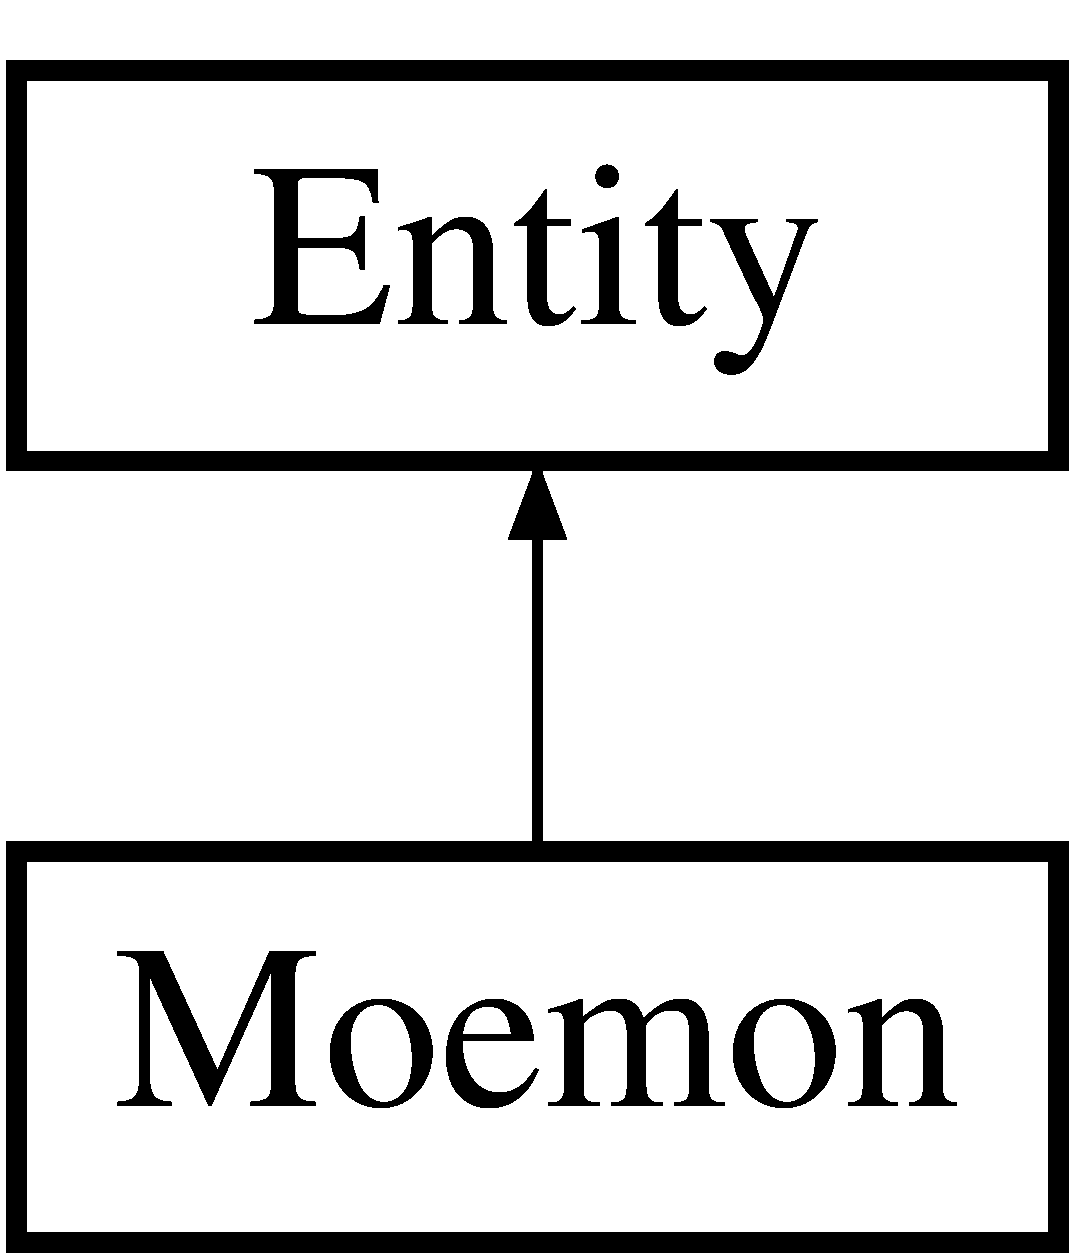
\includegraphics[height=2.000000cm]{class_moemon}
\end{center}
\end{figure}
\subsection*{Public Member Functions}
\begin{DoxyCompactItemize}
\item 
\hyperlink{class_moemon_a97eba25498b958c11e237c6e4bd868b2}{Moemon} (int id, int health, int attack, int defense, int Sp\+Atk, int Sp\+Def, int Speed, int level, std\+::string name, std\+::string type)
\begin{DoxyCompactList}\small\item\em The constructor of the Moe\+Mon object. \end{DoxyCompactList}\end{DoxyCompactItemize}
\subsection*{Additional Inherited Members}


\subsection{Detailed Description}
Class that represents an Moe\+Mon. 

This class contains the data that makes up a Moe\+Mon. It inherits from \hyperlink{class_entity}{Entity}, which assigns it a surface and texture. The data will be inputed from a file. 

\subsection{Constructor \& Destructor Documentation}
\hypertarget{class_moemon_a97eba25498b958c11e237c6e4bd868b2}{\index{Moemon@{Moemon}!Moemon@{Moemon}}
\index{Moemon@{Moemon}!Moemon@{Moemon}}
\subsubsection[{Moemon}]{\setlength{\rightskip}{0pt plus 5cm}Moemon\+::\+Moemon (
\begin{DoxyParamCaption}
\item[{int}]{id, }
\item[{int}]{health, }
\item[{int}]{attack, }
\item[{int}]{defense, }
\item[{int}]{Sp\+Atk, }
\item[{int}]{Sp\+Def, }
\item[{int}]{Speed, }
\item[{int}]{level, }
\item[{std\+::string}]{name, }
\item[{std\+::string}]{type}
\end{DoxyParamCaption}
)}}\label{class_moemon_a97eba25498b958c11e237c6e4bd868b2}


The constructor of the Moe\+Mon object. 

Constructs the Moe\+Mon from data that is read in from a file.


\begin{DoxyParams}{Parameters}
{\em int} & -\/ Contains the \hyperlink{class_moemon}{Moemon} id \\
\hline
{\em int} & -\/ Contains the \hyperlink{class_moemon}{Moemon} base health \\
\hline
{\em int} & -\/ Contains the \hyperlink{class_moemon}{Moemon} base attack \\
\hline
{\em int} & -\/ Contains the \hyperlink{class_moemon}{Moemon} base defense \\
\hline
{\em int} & -\/ Contains the \hyperlink{class_moemon}{Moemon} base Sp\+Atk \\
\hline
{\em int} & -\/ Contains the \hyperlink{class_moemon}{Moemon} base Sp\+Def \\
\hline
{\em int} & -\/ Contains the \hyperlink{class_moemon}{Moemon} base Speed \\
\hline
{\em int} & -\/ Contains the \hyperlink{class_moemon}{Moemon} default level \\
\hline
{\em std\+::string} & -\/ Contains the \hyperlink{class_moemon}{Moemon}'s name \\
\hline
{\em std\+::string} & -\/ Contains the \hyperlink{class_moemon}{Moemon}'s type \\
\hline
\end{DoxyParams}


The documentation for this class was generated from the following files\+:\begin{DoxyCompactItemize}
\item 
S\+D\+L/Moemon.\+h\item 
S\+D\+L/Moemon.\+cpp\end{DoxyCompactItemize}

\hypertarget{class_player}{\section{Player Class Reference}
\label{class_player}\index{Player@{Player}}
}


A class that represents a \hyperlink{class_player}{Player}.  




{\ttfamily \#include $<$Player.\+h$>$}

Inheritance diagram for Player\+:\begin{figure}[H]
\begin{center}
\leavevmode
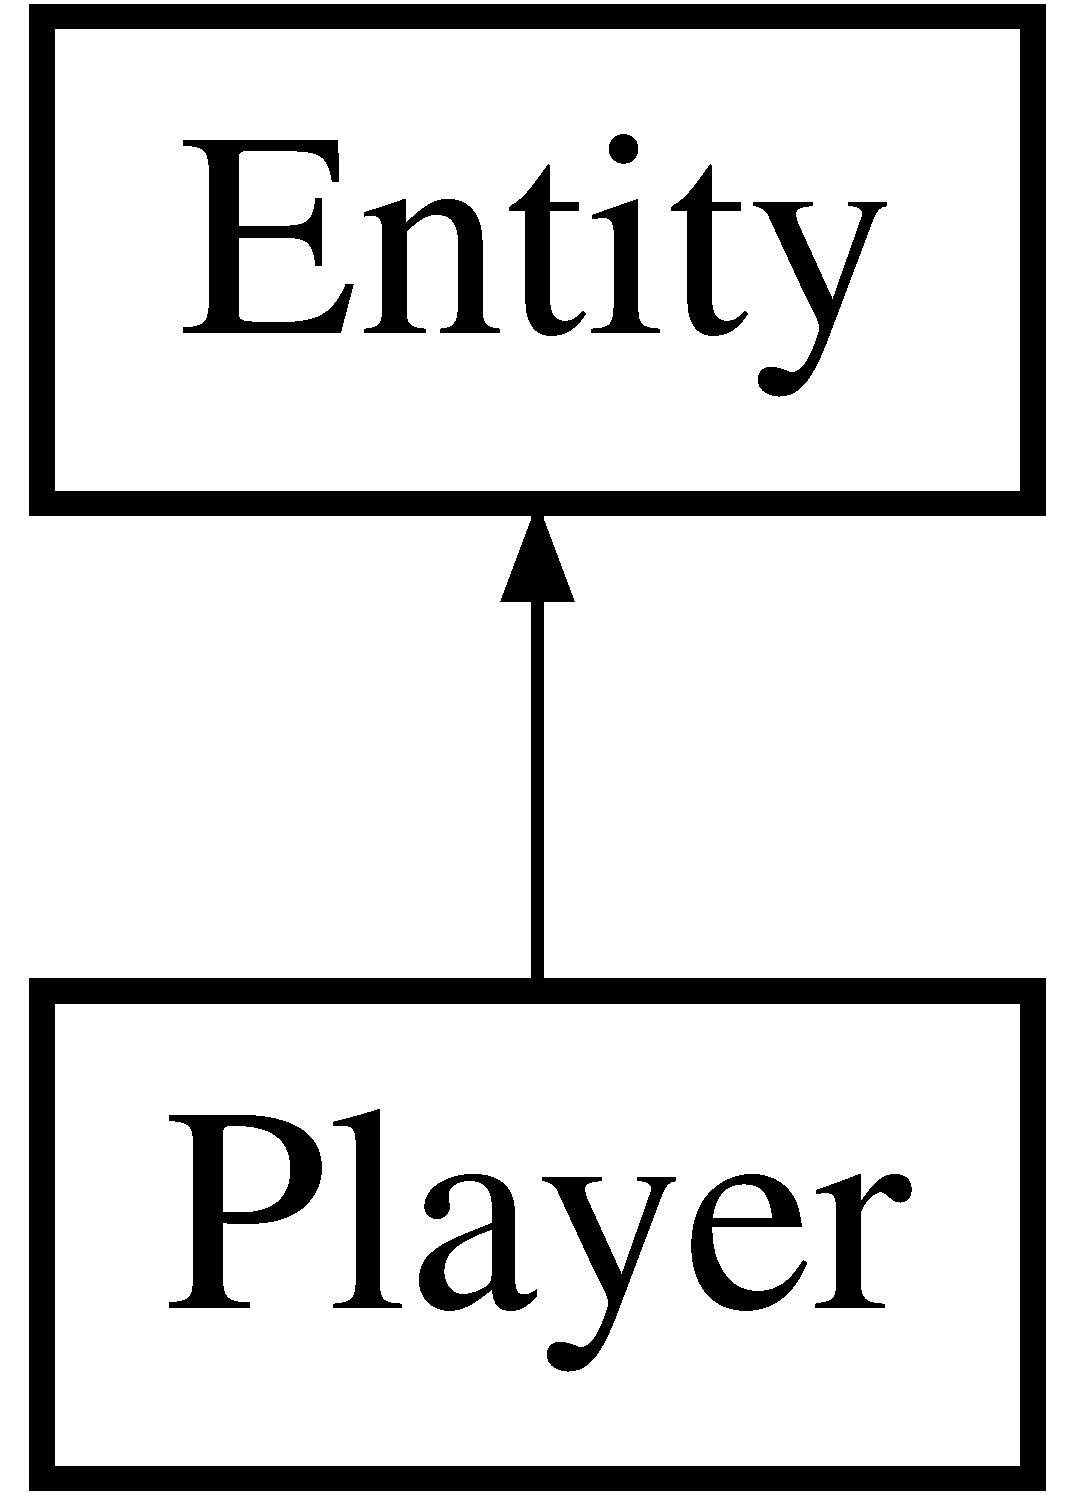
\includegraphics[height=2.000000cm]{class_player}
\end{center}
\end{figure}
\subsection*{Public Member Functions}
\begin{DoxyCompactItemize}
\item 
\hyperlink{class_player_a6cfff646e006e196fc4c125b3855fda3}{Player} (\hyperlink{struct_rect}{Rect} v1, \hyperlink{struct_rect}{Rect} sr1, float s)
\begin{DoxyCompactList}\small\item\em The player constructor. \end{DoxyCompactList}\item 
void \hyperlink{class_player_ab166e86a297493b2274851cec66b7ebc}{call\+Move\+Up} (bool can\+Move, \hyperlink{class_timer}{Timer} $\ast$Player\+Anim, \hyperlink{class_time}{Time} dt)
\begin{DoxyCompactList}\small\item\em A method for calling the player to move up. \end{DoxyCompactList}\item 
void \hyperlink{class_player_aab2dfd7d954c02ff3f39dc0de9d7b10b}{call\+Move\+Left} (bool can\+Move, \hyperlink{class_timer}{Timer} $\ast$Player\+Anim, \hyperlink{class_time}{Time} dt)
\begin{DoxyCompactList}\small\item\em A method for calling the player to move left. \end{DoxyCompactList}\item 
void \hyperlink{class_player_a6aa7f8a3b50732b365aed7e4d0685953}{call\+Move\+Right} (bool can\+Move, \hyperlink{class_timer}{Timer} $\ast$Player\+Anim, \hyperlink{class_time}{Time} dt)
\begin{DoxyCompactList}\small\item\em A method for calling the player to move right. \end{DoxyCompactList}\item 
void \hyperlink{class_player_a98cf56ce518c65de588c92464f1e6b2c}{call\+Move\+Down} (bool can\+Move, \hyperlink{class_timer}{Timer} $\ast$Player\+Anim, \hyperlink{class_time}{Time} dt)
\begin{DoxyCompactList}\small\item\em A method for calling the player to move down. \end{DoxyCompactList}\end{DoxyCompactItemize}
\subsection*{Additional Inherited Members}


\subsection{Detailed Description}
A class that represents a \hyperlink{class_player}{Player}. 

This class is a derived class of \hyperlink{class_entity}{Entity}, and is used to create the \hyperlink{class_player}{Player} object. 

\subsection{Constructor \& Destructor Documentation}
\hypertarget{class_player_a6cfff646e006e196fc4c125b3855fda3}{\index{Player@{Player}!Player@{Player}}
\index{Player@{Player}!Player@{Player}}
\subsubsection[{Player}]{\setlength{\rightskip}{0pt plus 5cm}Player\+::\+Player (
\begin{DoxyParamCaption}
\item[{{\bf Rect}}]{v1, }
\item[{{\bf Rect}}]{sr1, }
\item[{float}]{s}
\end{DoxyParamCaption}
)}}\label{class_player_a6cfff646e006e196fc4c125b3855fda3}


The player constructor. 


\begin{DoxyParams}{Parameters}
{\em \hyperlink{struct_rect}{Rect}} & -\/ A rect structure containing four floating point numbers for destination \\
\hline
{\em \hyperlink{struct_rect}{Rect}} & -\/ A rect structure containing four floating point numbers for source \\
\hline
{\em float} & -\/ A float containing the speed \\
\hline
\end{DoxyParams}


\subsection{Member Function Documentation}
\hypertarget{class_player_a98cf56ce518c65de588c92464f1e6b2c}{\index{Player@{Player}!call\+Move\+Down@{call\+Move\+Down}}
\index{call\+Move\+Down@{call\+Move\+Down}!Player@{Player}}
\subsubsection[{call\+Move\+Down}]{\setlength{\rightskip}{0pt plus 5cm}void Player\+::call\+Move\+Down (
\begin{DoxyParamCaption}
\item[{bool}]{can\+Move, }
\item[{{\bf Timer} $\ast$}]{Player\+Anim, }
\item[{{\bf Time}}]{dt}
\end{DoxyParamCaption}
)}}\label{class_player_a98cf56ce518c65de588c92464f1e6b2c}


A method for calling the player to move down. 


\begin{DoxyParams}{Parameters}
{\em bool} & -\/ A bool containing a true/false if the player can move \\
\hline
{\em Timer$\ast$} & -\/ A timer to control the player's animation \\
\hline
{\em \hyperlink{class_time}{Time}} & -\/ The time for accessing time method (e.\+g. Delta time) \\
\hline
\end{DoxyParams}
dt.\+get\+Delta() \hypertarget{class_player_aab2dfd7d954c02ff3f39dc0de9d7b10b}{\index{Player@{Player}!call\+Move\+Left@{call\+Move\+Left}}
\index{call\+Move\+Left@{call\+Move\+Left}!Player@{Player}}
\subsubsection[{call\+Move\+Left}]{\setlength{\rightskip}{0pt plus 5cm}void Player\+::call\+Move\+Left (
\begin{DoxyParamCaption}
\item[{bool}]{can\+Move, }
\item[{{\bf Timer} $\ast$}]{Player\+Anim, }
\item[{{\bf Time}}]{dt}
\end{DoxyParamCaption}
)}}\label{class_player_aab2dfd7d954c02ff3f39dc0de9d7b10b}


A method for calling the player to move left. 


\begin{DoxyParams}{Parameters}
{\em bool} & -\/ A bool containing a true/false if the player can move \\
\hline
{\em Timer$\ast$} & -\/ A timer to control the player's animation \\
\hline
{\em \hyperlink{class_time}{Time}} & -\/ The time for accessing time method (e.\+g. Delta time) \\
\hline
\end{DoxyParams}
dt.\+get\+Delta() \hypertarget{class_player_a6aa7f8a3b50732b365aed7e4d0685953}{\index{Player@{Player}!call\+Move\+Right@{call\+Move\+Right}}
\index{call\+Move\+Right@{call\+Move\+Right}!Player@{Player}}
\subsubsection[{call\+Move\+Right}]{\setlength{\rightskip}{0pt plus 5cm}void Player\+::call\+Move\+Right (
\begin{DoxyParamCaption}
\item[{bool}]{can\+Move, }
\item[{{\bf Timer} $\ast$}]{Player\+Anim, }
\item[{{\bf Time}}]{dt}
\end{DoxyParamCaption}
)}}\label{class_player_a6aa7f8a3b50732b365aed7e4d0685953}


A method for calling the player to move right. 


\begin{DoxyParams}{Parameters}
{\em bool} & -\/ A bool containing a true/false if the player can move \\
\hline
{\em Timer$\ast$} & -\/ A timer to control the player's animation \\
\hline
{\em \hyperlink{class_time}{Time}} & -\/ The time for accessing time method (e.\+g. Delta time) \\
\hline
\end{DoxyParams}
dt.\+get\+Delta() \hypertarget{class_player_ab166e86a297493b2274851cec66b7ebc}{\index{Player@{Player}!call\+Move\+Up@{call\+Move\+Up}}
\index{call\+Move\+Up@{call\+Move\+Up}!Player@{Player}}
\subsubsection[{call\+Move\+Up}]{\setlength{\rightskip}{0pt plus 5cm}void Player\+::call\+Move\+Up (
\begin{DoxyParamCaption}
\item[{bool}]{can\+Move, }
\item[{{\bf Timer} $\ast$}]{Player\+Anim, }
\item[{{\bf Time}}]{dt}
\end{DoxyParamCaption}
)}}\label{class_player_ab166e86a297493b2274851cec66b7ebc}


A method for calling the player to move up. 


\begin{DoxyParams}{Parameters}
{\em bool} & -\/ A bool containing a true/false if the player can move \\
\hline
{\em Timer$\ast$} & -\/ A timer to control the player's animation \\
\hline
{\em \hyperlink{class_time}{Time}} & -\/ The time for accessing time method (e.\+g. Delta time) \\
\hline
\end{DoxyParams}
dt.\+get\+Delta() 

The documentation for this class was generated from the following files\+:\begin{DoxyCompactItemize}
\item 
S\+D\+L/Player.\+h\item 
S\+D\+L/Player.\+cpp\end{DoxyCompactItemize}

\hypertarget{struct_rect}{\section{Rect Struct Reference}
\label{struct_rect}\index{Rect@{Rect}}
}


A structure containing four floats.  




{\ttfamily \#include $<$Source\+Rect.\+h$>$}

\subsection*{Public Member Functions}
\begin{DoxyCompactItemize}
\item 
\hyperlink{struct_rect_a21e3f21b1579b6aea19ea88d89c019ef}{Rect} (float x, float y, float w, float h)
\begin{DoxyCompactList}\small\item\em A constructor for the structure that takes in four parameters. \end{DoxyCompactList}\end{DoxyCompactItemize}
\subsection*{Public Attributes}
\begin{DoxyCompactItemize}
\item 
\hypertarget{struct_rect_afbb60a370ff89951ddad6ff377e75a94}{float {\bfseries f\+\_\+x}}\label{struct_rect_afbb60a370ff89951ddad6ff377e75a94}

\item 
\hypertarget{struct_rect_a12b49f1cb04bf92f77dde91f53bf99d8}{float {\bfseries f\+\_\+y}}\label{struct_rect_a12b49f1cb04bf92f77dde91f53bf99d8}

\item 
\hypertarget{struct_rect_a6cc260d7e6d6fd07514cd88ac785e0f6}{float {\bfseries f\+\_\+w}}\label{struct_rect_a6cc260d7e6d6fd07514cd88ac785e0f6}

\item 
\hypertarget{struct_rect_a784fe78544bcb8705e652d3a8eaa4a86}{float {\bfseries f\+\_\+h}}\label{struct_rect_a784fe78544bcb8705e652d3a8eaa4a86}

\end{DoxyCompactItemize}


\subsection{Detailed Description}
A structure containing four floats. 

This structure is used for creating Source Rects for sprite maps 

\subsection{Constructor \& Destructor Documentation}
\hypertarget{struct_rect_a21e3f21b1579b6aea19ea88d89c019ef}{\index{Rect@{Rect}!Rect@{Rect}}
\index{Rect@{Rect}!Rect@{Rect}}
\subsubsection[{Rect}]{\setlength{\rightskip}{0pt plus 5cm}Rect\+::\+Rect (
\begin{DoxyParamCaption}
\item[{float}]{x, }
\item[{float}]{y, }
\item[{float}]{w, }
\item[{float}]{h}
\end{DoxyParamCaption}
)\hspace{0.3cm}{\ttfamily [inline]}}}\label{struct_rect_a21e3f21b1579b6aea19ea88d89c019ef}


A constructor for the structure that takes in four parameters. 


\begin{DoxyParams}{Parameters}
{\em float} & -\/ A float containing the x axises \\
\hline
{\em float} & -\/ A float containing the y axises \\
\hline
{\em float} & -\/ A float containing the width \\
\hline
{\em float} & -\/ A float containing the height \\
\hline
\end{DoxyParams}


The documentation for this struct was generated from the following file\+:\begin{DoxyCompactItemize}
\item 
S\+D\+L/Source\+Rect.\+h\end{DoxyCompactItemize}

\hypertarget{class_texture}{\section{Texture Class Reference}
\label{class_texture}\index{Texture@{Texture}}
}
\subsection*{Public Member Functions}
\begin{DoxyCompactItemize}
\item 
\hypertarget{class_texture_aae2ae5192935d618e4f9de8d94bd89fd}{{\bfseries Texture} (std\+::string path, int, int)}\label{class_texture_aae2ae5192935d618e4f9de8d94bd89fd}

\item 
\hypertarget{class_texture_a28ddeead9d09927584663c5d2d582df2}{bool {\bfseries load\+From\+File} (std\+::string path)}\label{class_texture_a28ddeead9d09927584663c5d2d582df2}

\item 
\hypertarget{class_texture_a51f7aa720b0f538ee4dc9643d25b9fc5}{void {\bfseries Deallocate} ()}\label{class_texture_a51f7aa720b0f538ee4dc9643d25b9fc5}

\item 
\hypertarget{class_texture_a430b8ba2a5d32306903058de1bde5657}{void {\bfseries set\+Colour} (S\+D\+L\+\_\+\+Renderer $\ast$Back\+Renderer)}\label{class_texture_a430b8ba2a5d32306903058de1bde5657}

\item 
\hypertarget{class_texture_a560712606c4dc416722acf191250fddc}{void {\bfseries clear} (S\+D\+L\+\_\+\+Renderer $\ast$Back\+Renderer)}\label{class_texture_a560712606c4dc416722acf191250fddc}

\item 
\hypertarget{class_texture_ac2a59a47cceb887b1eb82788346690ad}{void {\bfseries set\+Alpha} ()}\label{class_texture_ac2a59a47cceb887b1eb82788346690ad}

\item 
\hypertarget{class_texture_a6858c96df93d340c8612cc67b038717b}{void {\bfseries Render} (S\+D\+L\+\_\+\+Renderer $\ast$Back\+Renderer)}\label{class_texture_a6858c96df93d340c8612cc67b038717b}

\item 
\hypertarget{class_texture_ad42de0731a4e4882a08b3c703807d8bb}{void {\bfseries Copy\+To\+Screen} (S\+D\+L\+\_\+\+Renderer $\ast$Back\+Renderer)}\label{class_texture_ad42de0731a4e4882a08b3c703807d8bb}

\item 
\hypertarget{class_texture_aa15e62be772d329c2e9d49d4d3bc056d}{void {\bfseries Show\+Screen} (S\+D\+L\+\_\+\+Renderer $\ast$Back\+Renderer)}\label{class_texture_aa15e62be772d329c2e9d49d4d3bc056d}

\item 
\hypertarget{class_texture_ab16f87249854565e57dea04d5340e749}{void {\bfseries Qurey\+Texture} ()}\label{class_texture_ab16f87249854565e57dea04d5340e749}

\item 
\hypertarget{class_texture_a25de7f57b9c0f5d118dbbff4658e7ea3}{void {\bfseries Process\+Texture} (S\+D\+L\+\_\+\+Renderer $\ast$Back\+Renderer)}\label{class_texture_a25de7f57b9c0f5d118dbbff4658e7ea3}

\end{DoxyCompactItemize}
\subsection*{Protected Attributes}
\begin{DoxyCompactItemize}
\item 
\hypertarget{class_texture_a6a3681af920ae2d2d7dea0317e817b91}{S\+D\+L\+\_\+\+Texture $\ast$ {\bfseries c\+Texture}}\label{class_texture_a6a3681af920ae2d2d7dea0317e817b91}

\item 
\hypertarget{class_texture_a383889ec8959fbbdcd47f7ab2fd86fa0}{S\+D\+L\+\_\+\+Surface $\ast$ {\bfseries c\+Image}}\label{class_texture_a383889ec8959fbbdcd47f7ab2fd86fa0}

\item 
\hypertarget{class_texture_a21602e597acc6851d97701187cab01b1}{S\+D\+L\+\_\+\+Rect {\bfseries c\+Dest\+Rect}}\label{class_texture_a21602e597acc6851d97701187cab01b1}

\item 
\hypertarget{class_texture_accab810fad8662a19ec8ce15316e0e6e}{int {\bfseries i\+Width}}\label{class_texture_accab810fad8662a19ec8ce15316e0e6e}

\item 
\hypertarget{class_texture_a23ce6d3594246ffd6c794c14a328ba83}{int {\bfseries i\+Height}}\label{class_texture_a23ce6d3594246ffd6c794c14a328ba83}

\end{DoxyCompactItemize}


The documentation for this class was generated from the following files\+:\begin{DoxyCompactItemize}
\item 
S\+D\+L/Texture.\+h\item 
S\+D\+L/Texture.\+cpp\end{DoxyCompactItemize}

\hypertarget{class_tile}{\section{Tile Class Reference}
\label{class_tile}\index{Tile@{Tile}}
}


A class that represents a \hyperlink{class_tile}{Tile}.  




{\ttfamily \#include $<$Tile.\+h$>$}

\subsection*{Public Member Functions}
\begin{DoxyCompactItemize}
\item 
\hypertarget{class_tile_aeeb5593bb6b75aae2edfcccbc84ab378}{\hyperlink{class_tile_aeeb5593bb6b75aae2edfcccbc84ab378}{Tile} ()}\label{class_tile_aeeb5593bb6b75aae2edfcccbc84ab378}

\begin{DoxyCompactList}\small\item\em The default constructor for the \hyperlink{class_tile}{Tile} object. \end{DoxyCompactList}\item 
\hyperlink{class_tile_af825c40b67f4d0544c29f294363919a8}{Tile} (int x, int y, int type)
\begin{DoxyCompactList}\small\item\em The constructor for the \hyperlink{class_tile}{Tile} object. \end{DoxyCompactList}\item 
\hypertarget{class_tile_a98634abbd93fa13d0578d7103202d03d}{\hyperlink{class_tile_a98634abbd93fa13d0578d7103202d03d}{$\sim$\+Tile} ()}\label{class_tile_a98634abbd93fa13d0578d7103202d03d}

\begin{DoxyCompactList}\small\item\em The deconstructor for the \hyperlink{class_tile}{Tile} object. \end{DoxyCompactList}\item 
int \hyperlink{class_tile_a8582d28ecc7a974dd6d5263d73b8f1f1}{get\+Type} ()
\begin{DoxyCompactList}\small\item\em A method to get the type of tile. \end{DoxyCompactList}\item 
S\+D\+L\+\_\+\+Rect \hyperlink{class_tile_a80c85e60ea0a0dc196fb5ebed132e386}{get\+Box} ()
\begin{DoxyCompactList}\small\item\em A method to get the S\+D\+L\+\_\+\+Rect of the tile. \end{DoxyCompactList}\end{DoxyCompactItemize}


\subsection{Detailed Description}
A class that represents a \hyperlink{class_tile}{Tile}. 

This class is used to create tile objects 

\subsection{Constructor \& Destructor Documentation}
\hypertarget{class_tile_af825c40b67f4d0544c29f294363919a8}{\index{Tile@{Tile}!Tile@{Tile}}
\index{Tile@{Tile}!Tile@{Tile}}
\subsubsection[{Tile}]{\setlength{\rightskip}{0pt plus 5cm}Tile\+::\+Tile (
\begin{DoxyParamCaption}
\item[{int}]{x, }
\item[{int}]{y, }
\item[{int}]{type}
\end{DoxyParamCaption}
)}}\label{class_tile_af825c40b67f4d0544c29f294363919a8}


The constructor for the \hyperlink{class_tile}{Tile} object. 


\begin{DoxyParams}{Parameters}
{\em int} & -\/ An int containing the x axises \\
\hline
{\em int} & -\/ An int containing the y axises \\
\hline
{\em int} & -\/ An int containing the type of tile \\
\hline
\end{DoxyParams}


\subsection{Member Function Documentation}
\hypertarget{class_tile_a80c85e60ea0a0dc196fb5ebed132e386}{\index{Tile@{Tile}!get\+Box@{get\+Box}}
\index{get\+Box@{get\+Box}!Tile@{Tile}}
\subsubsection[{get\+Box}]{\setlength{\rightskip}{0pt plus 5cm}S\+D\+L\+\_\+\+Rect Tile\+::get\+Box (
\begin{DoxyParamCaption}
{}
\end{DoxyParamCaption}
)}}\label{class_tile_a80c85e60ea0a0dc196fb5ebed132e386}


A method to get the S\+D\+L\+\_\+\+Rect of the tile. 

Returns a S\+D\+L\+\_\+\+Rect. \begin{DoxyReturn}{Returns}
S\+D\+L\+\_\+\+Rect 
\end{DoxyReturn}
\hypertarget{class_tile_a8582d28ecc7a974dd6d5263d73b8f1f1}{\index{Tile@{Tile}!get\+Type@{get\+Type}}
\index{get\+Type@{get\+Type}!Tile@{Tile}}
\subsubsection[{get\+Type}]{\setlength{\rightskip}{0pt plus 5cm}int Tile\+::get\+Type (
\begin{DoxyParamCaption}
{}
\end{DoxyParamCaption}
)}}\label{class_tile_a8582d28ecc7a974dd6d5263d73b8f1f1}


A method to get the type of tile. 

Returns an int that relates to what type the tile is. \begin{DoxyReturn}{Returns}
int -\/ Containing type 
\end{DoxyReturn}


The documentation for this class was generated from the following files\+:\begin{DoxyCompactItemize}
\item 
S\+D\+L/Tile.\+h\item 
S\+D\+L/Tile.\+cpp\end{DoxyCompactItemize}

\hypertarget{class_time}{\section{Time Class Reference}
\label{class_time}\index{Time@{Time}}
}


A class that represents time.  




{\ttfamily \#include $<$Time.\+h$>$}

\subsection*{Public Member Functions}
\begin{DoxyCompactItemize}
\item 
\hypertarget{class_time_a4245e409c7347d1d671858962c2ca3b5}{\hyperlink{class_time_a4245e409c7347d1d671858962c2ca3b5}{Time} ()}\label{class_time_a4245e409c7347d1d671858962c2ca3b5}

\begin{DoxyCompactList}\small\item\em The time class object constructor. \end{DoxyCompactList}\item 
\hypertarget{class_time_a1e92dbe963fa3cdd6bea207680f5f6d1}{\hyperlink{class_time_a1e92dbe963fa3cdd6bea207680f5f6d1}{$\sim$\+Time} ()}\label{class_time_a1e92dbe963fa3cdd6bea207680f5f6d1}

\begin{DoxyCompactList}\small\item\em The time class object deconstructor. \end{DoxyCompactList}\item 
void \hyperlink{class_time_a8207bba903bd8da8bc1b27e10f1fc67a}{call\+Start} ()
\begin{DoxyCompactList}\small\item\em A method to call the start of the time class. \end{DoxyCompactList}\item 
void \hyperlink{class_time_a1a2c7ad114dcf149aa41115f725080d4}{call\+Pause} ()
\begin{DoxyCompactList}\small\item\em A method to call the time pause. \end{DoxyCompactList}\item 
void \hyperlink{class_time_a4eb1dba53fb0189db133c2e6e93b7fc0}{call\+Unpause} ()
\begin{DoxyCompactList}\small\item\em A method to call the time unpause. \end{DoxyCompactList}\item 
void \hyperlink{class_time_a4481e9a19672b1587d6d429cf9f79b58}{call\+Stop} ()
\begin{DoxyCompactList}\small\item\em A method to call time stop. \end{DoxyCompactList}\item 
float \hyperlink{class_time_a9ad8743ccda87310ab3370aaf75c304e}{get\+Delta} ()
\begin{DoxyCompactList}\small\item\em A method to get the delta time. \end{DoxyCompactList}\item 
void \hyperlink{class_time_a6ca53f2e34d612ffb44e94b35186614b}{update\+Time} ()
\begin{DoxyCompactList}\small\item\em A method to update the time. \end{DoxyCompactList}\item 
bool \hyperlink{class_time_afebb5bb24dcb1ce79b99c9d64684d514}{is\+Paused} ()
\begin{DoxyCompactList}\small\item\em A method to check if the time is paused. \end{DoxyCompactList}\item 
bool \hyperlink{class_time_a85dce372c94fb3b773d77fc731998a16}{is\+Started} ()
\begin{DoxyCompactList}\small\item\em A method to check if the time has started. \end{DoxyCompactList}\end{DoxyCompactItemize}


\subsection{Detailed Description}
A class that represents time. 

This class is used to create a time object that is used for update functions/methods. 

\subsection{Member Function Documentation}
\hypertarget{class_time_a1a2c7ad114dcf149aa41115f725080d4}{\index{Time@{Time}!call\+Pause@{call\+Pause}}
\index{call\+Pause@{call\+Pause}!Time@{Time}}
\subsubsection[{call\+Pause}]{\setlength{\rightskip}{0pt plus 5cm}void Time\+::call\+Pause (
\begin{DoxyParamCaption}
{}
\end{DoxyParamCaption}
)}}\label{class_time_a1a2c7ad114dcf149aa41115f725080d4}


A method to call the time pause. 

Pauses the time. \hypertarget{class_time_a8207bba903bd8da8bc1b27e10f1fc67a}{\index{Time@{Time}!call\+Start@{call\+Start}}
\index{call\+Start@{call\+Start}!Time@{Time}}
\subsubsection[{call\+Start}]{\setlength{\rightskip}{0pt plus 5cm}void Time\+::call\+Start (
\begin{DoxyParamCaption}
{}
\end{DoxyParamCaption}
)}}\label{class_time_a8207bba903bd8da8bc1b27e10f1fc67a}


A method to call the start of the time class. 

Starts the time, and to be used on application initialisation. \hypertarget{class_time_a4481e9a19672b1587d6d429cf9f79b58}{\index{Time@{Time}!call\+Stop@{call\+Stop}}
\index{call\+Stop@{call\+Stop}!Time@{Time}}
\subsubsection[{call\+Stop}]{\setlength{\rightskip}{0pt plus 5cm}void Time\+::call\+Stop (
\begin{DoxyParamCaption}
{}
\end{DoxyParamCaption}
)}}\label{class_time_a4481e9a19672b1587d6d429cf9f79b58}


A method to call time stop. 

Stops the time completely. \hypertarget{class_time_a4eb1dba53fb0189db133c2e6e93b7fc0}{\index{Time@{Time}!call\+Unpause@{call\+Unpause}}
\index{call\+Unpause@{call\+Unpause}!Time@{Time}}
\subsubsection[{call\+Unpause}]{\setlength{\rightskip}{0pt plus 5cm}void Time\+::call\+Unpause (
\begin{DoxyParamCaption}
{}
\end{DoxyParamCaption}
)}}\label{class_time_a4eb1dba53fb0189db133c2e6e93b7fc0}


A method to call the time unpause. 

Unpauses the time. \hypertarget{class_time_a9ad8743ccda87310ab3370aaf75c304e}{\index{Time@{Time}!get\+Delta@{get\+Delta}}
\index{get\+Delta@{get\+Delta}!Time@{Time}}
\subsubsection[{get\+Delta}]{\setlength{\rightskip}{0pt plus 5cm}float Time\+::get\+Delta (
\begin{DoxyParamCaption}
{}
\end{DoxyParamCaption}
)}}\label{class_time_a9ad8743ccda87310ab3370aaf75c304e}


A method to get the delta time. 

Returns a float that contains delta time. \hypertarget{class_time_afebb5bb24dcb1ce79b99c9d64684d514}{\index{Time@{Time}!is\+Paused@{is\+Paused}}
\index{is\+Paused@{is\+Paused}!Time@{Time}}
\subsubsection[{is\+Paused}]{\setlength{\rightskip}{0pt plus 5cm}bool Time\+::is\+Paused (
\begin{DoxyParamCaption}
{}
\end{DoxyParamCaption}
)}}\label{class_time_afebb5bb24dcb1ce79b99c9d64684d514}


A method to check if the time is paused. 

Returns a true/false if the application is paused. \begin{DoxyReturn}{Returns}
bool 
\end{DoxyReturn}
\hypertarget{class_time_a85dce372c94fb3b773d77fc731998a16}{\index{Time@{Time}!is\+Started@{is\+Started}}
\index{is\+Started@{is\+Started}!Time@{Time}}
\subsubsection[{is\+Started}]{\setlength{\rightskip}{0pt plus 5cm}bool Time\+::is\+Started (
\begin{DoxyParamCaption}
{}
\end{DoxyParamCaption}
)}}\label{class_time_a85dce372c94fb3b773d77fc731998a16}


A method to check if the time has started. 

Returns a true/false if the application time is unpaused. \begin{DoxyReturn}{Returns}
bool 
\end{DoxyReturn}
\hypertarget{class_time_a6ca53f2e34d612ffb44e94b35186614b}{\index{Time@{Time}!update\+Time@{update\+Time}}
\index{update\+Time@{update\+Time}!Time@{Time}}
\subsubsection[{update\+Time}]{\setlength{\rightskip}{0pt plus 5cm}void Time\+::update\+Time (
\begin{DoxyParamCaption}
{}
\end{DoxyParamCaption}
)}}\label{class_time_a6ca53f2e34d612ffb44e94b35186614b}


A method to update the time. 

Called in the application loop to constantly update time. \begin{DoxyReturn}{Returns}
float -\/ Containing Delta \hyperlink{class_time}{Time} 
\end{DoxyReturn}


The documentation for this class was generated from the following files\+:\begin{DoxyCompactItemize}
\item 
S\+D\+L/Time.\+h\item 
S\+D\+L/Time.\+cpp\end{DoxyCompactItemize}

\hypertarget{class_timer}{\section{Timer Class Reference}
\label{class_timer}\index{Timer@{Timer}}
}


A class that represents a timer.  




{\ttfamily \#include $<$Timer.\+h$>$}

\subsection*{Public Member Functions}
\begin{DoxyCompactItemize}
\item 
\hyperlink{class_timer_a2cf265defc892796c92dc09d8a482ced}{Timer} (float ms)
\begin{DoxyCompactList}\small\item\em The timer class object constructor. \end{DoxyCompactList}\item 
\hyperlink{class_timer_a14fa469c4c295c5fa6e66a4ad1092146}{$\sim$\+Timer} ()
\begin{DoxyCompactList}\small\item\em The time class object deconstructor. \end{DoxyCompactList}\item 
void \hyperlink{class_timer_a796907a264f364f5a4c819e7c18b1302}{update\+Timer} (float Delta\+Time)
\begin{DoxyCompactList}\small\item\em A method for updating the timer. \end{DoxyCompactList}\item 
bool \hyperlink{class_timer_a3ddc2b42f18cae583dc1a730fbd29fac}{expired\+Timer} ()
\begin{DoxyCompactList}\small\item\em A method for checking if the time has expired. \end{DoxyCompactList}\item 
int \hyperlink{class_timer_a32b0f17af4c43fc9a6f9730c718d1f9d}{debug} ()
\begin{DoxyCompactList}\small\item\em A debug method for timer. \end{DoxyCompactList}\end{DoxyCompactItemize}


\subsection{Detailed Description}
A class that represents a timer. 

This class is used to create timers that take in the delta time, and checks if the timer has expired. 

\subsection{Constructor \& Destructor Documentation}
\hypertarget{class_timer_a2cf265defc892796c92dc09d8a482ced}{\index{Timer@{Timer}!Timer@{Timer}}
\index{Timer@{Timer}!Timer@{Timer}}
\subsubsection[{Timer}]{\setlength{\rightskip}{0pt plus 5cm}Timer\+::\+Timer (
\begin{DoxyParamCaption}
\item[{float}]{ms}
\end{DoxyParamCaption}
)}}\label{class_timer_a2cf265defc892796c92dc09d8a482ced}


The timer class object constructor. 

Takes in a float parameter to set up the timer. 
\begin{DoxyParams}{Parameters}
{\em float} & -\/ \hyperlink{class_time}{Time} for the timer \\
\hline
\end{DoxyParams}
\hypertarget{class_timer_a14fa469c4c295c5fa6e66a4ad1092146}{\index{Timer@{Timer}!````~Timer@{$\sim$\+Timer}}
\index{````~Timer@{$\sim$\+Timer}!Timer@{Timer}}
\subsubsection[{$\sim$\+Timer}]{\setlength{\rightskip}{0pt plus 5cm}Timer\+::$\sim$\+Timer (
\begin{DoxyParamCaption}
{}
\end{DoxyParamCaption}
)}}\label{class_timer_a14fa469c4c295c5fa6e66a4ad1092146}


The time class object deconstructor. 

Destroys the timer object 

\subsection{Member Function Documentation}
\hypertarget{class_timer_a32b0f17af4c43fc9a6f9730c718d1f9d}{\index{Timer@{Timer}!debug@{debug}}
\index{debug@{debug}!Timer@{Timer}}
\subsubsection[{debug}]{\setlength{\rightskip}{0pt plus 5cm}int Timer\+::debug (
\begin{DoxyParamCaption}
{}
\end{DoxyParamCaption}
)}}\label{class_timer_a32b0f17af4c43fc9a6f9730c718d1f9d}


A debug method for timer. 

Returns the timer's current value. \begin{DoxyReturn}{Returns}
int 
\end{DoxyReturn}
\hypertarget{class_timer_a3ddc2b42f18cae583dc1a730fbd29fac}{\index{Timer@{Timer}!expired\+Timer@{expired\+Timer}}
\index{expired\+Timer@{expired\+Timer}!Timer@{Timer}}
\subsubsection[{expired\+Timer}]{\setlength{\rightskip}{0pt plus 5cm}bool Timer\+::expired\+Timer (
\begin{DoxyParamCaption}
{}
\end{DoxyParamCaption}
)}}\label{class_timer_a3ddc2b42f18cae583dc1a730fbd29fac}


A method for checking if the time has expired. 

Checks if the timer has expired, and returns a true/false. \begin{DoxyReturn}{Returns}
bool 
\end{DoxyReturn}
\hypertarget{class_timer_a796907a264f364f5a4c819e7c18b1302}{\index{Timer@{Timer}!update\+Timer@{update\+Timer}}
\index{update\+Timer@{update\+Timer}!Timer@{Timer}}
\subsubsection[{update\+Timer}]{\setlength{\rightskip}{0pt plus 5cm}void Timer\+::update\+Timer (
\begin{DoxyParamCaption}
\item[{float}]{Delta\+Time}
\end{DoxyParamCaption}
)}}\label{class_timer_a796907a264f364f5a4c819e7c18b1302}


A method for updating the timer. 

Takes in the parameter of delta time to update the timer. 
\begin{DoxyParams}{Parameters}
{\em float} & -\/ A float containing the delta time \\
\hline
\end{DoxyParams}


The documentation for this class was generated from the following files\+:\begin{DoxyCompactItemize}
\item 
S\+D\+L/Timer.\+h\item 
S\+D\+L/Timer.\+cpp\end{DoxyCompactItemize}

\hypertarget{struct_vec2}{\section{Vec2 Struct Reference}
\label{struct_vec2}\index{Vec2@{Vec2}}
}


A structure that represents a Vector of 2 dimensions.  




{\ttfamily \#include $<$Vec2.\+h$>$}

\subsection*{Public Member Functions}
\begin{DoxyCompactItemize}
\item 
\hyperlink{struct_vec2_a6256fecebf5a43b14d5d5341c58cfdc4}{Vec2} (float x, float y)
\begin{DoxyCompactList}\small\item\em A constructor for the structure. \end{DoxyCompactList}\end{DoxyCompactItemize}
\subsection*{Public Attributes}
\begin{DoxyCompactItemize}
\item 
\hypertarget{struct_vec2_aacf790ce896c6730590b56a307a554c3}{float \hyperlink{struct_vec2_aacf790ce896c6730590b56a307a554c3}{f\+\_\+x}}\label{struct_vec2_aacf790ce896c6730590b56a307a554c3}

\begin{DoxyCompactList}\small\item\em Float that represents the X axises. \end{DoxyCompactList}\item 
\hypertarget{struct_vec2_ad4eb6792a7c62c9faed59702b60fe87a}{float \hyperlink{struct_vec2_ad4eb6792a7c62c9faed59702b60fe87a}{f\+\_\+y}}\label{struct_vec2_ad4eb6792a7c62c9faed59702b60fe87a}

\begin{DoxyCompactList}\small\item\em Float that represents the Y axises. \end{DoxyCompactList}\end{DoxyCompactItemize}


\subsection{Detailed Description}
A structure that represents a Vector of 2 dimensions. 

This structure contains two floating point numbers 

\subsection{Constructor \& Destructor Documentation}
\hypertarget{struct_vec2_a6256fecebf5a43b14d5d5341c58cfdc4}{\index{Vec2@{Vec2}!Vec2@{Vec2}}
\index{Vec2@{Vec2}!Vec2@{Vec2}}
\subsubsection[{Vec2}]{\setlength{\rightskip}{0pt plus 5cm}Vec2\+::\+Vec2 (
\begin{DoxyParamCaption}
\item[{float}]{x, }
\item[{float}]{y}
\end{DoxyParamCaption}
)\hspace{0.3cm}{\ttfamily [inline]}}}\label{struct_vec2_a6256fecebf5a43b14d5d5341c58cfdc4}


A constructor for the structure. 

Takes in two float parameters, and assigns them to x/y 
\begin{DoxyParams}{Parameters}
{\em float} & -\/ A float with the X axises \\
\hline
{\em float} & -\/ A float with the Y axises \\
\hline
\end{DoxyParams}


The documentation for this struct was generated from the following file\+:\begin{DoxyCompactItemize}
\item 
S\+D\+L/Vec2.\+h\end{DoxyCompactItemize}

\hypertarget{struct_vec4}{\section{Vec4 Struct Reference}
\label{struct_vec4}\index{Vec4@{Vec4}}
}
\subsection*{Public Member Functions}
\begin{DoxyCompactItemize}
\item 
\hypertarget{struct_vec4_a56a99878706317ae99f33cb9d94fadb0}{{\bfseries Vec4} (float x, float y, float w, float h)}\label{struct_vec4_a56a99878706317ae99f33cb9d94fadb0}

\end{DoxyCompactItemize}
\subsection*{Public Attributes}
\begin{DoxyCompactItemize}
\item 
\hypertarget{struct_vec4_aed4f75eeba3a5e32acc0eebee70ac1a6}{float {\bfseries f\+\_\+x}}\label{struct_vec4_aed4f75eeba3a5e32acc0eebee70ac1a6}

\item 
\hypertarget{struct_vec4_a9e6802ebe62f86c85994901f764ac0fc}{float {\bfseries f\+\_\+y}}\label{struct_vec4_a9e6802ebe62f86c85994901f764ac0fc}

\item 
\hypertarget{struct_vec4_a14b4beebb11d0a0daf201fe8e225e739}{float {\bfseries f\+\_\+w}}\label{struct_vec4_a14b4beebb11d0a0daf201fe8e225e739}

\item 
\hypertarget{struct_vec4_a34749726e12bb1258b6f2941fa60b7ed}{float {\bfseries f\+\_\+h}}\label{struct_vec4_a34749726e12bb1258b6f2941fa60b7ed}

\end{DoxyCompactItemize}


The documentation for this struct was generated from the following file\+:\begin{DoxyCompactItemize}
\item 
S\+D\+L/Vec4.\+h\end{DoxyCompactItemize}

%--- End generated contents ---

% Index
\newpage
\phantomsection
\addcontentsline{toc}{chapter}{Index}
\printindex

\end{document}
